\documentclass[oneside,final,a4paper]{report}

\usepackage{graphicx}
\usepackage{enumerate}
\usepackage[parfill]{parskip}
\usepackage[section]{placeins}
\usepackage{listings}

\graphicspath{{../report/images/} {../../www/mte481/website/static/} {./images/} {./appendices/}}

\lstset{language=C++}

\oddsidemargin 0in
\evensidemargin 0in
\textwidth 6.5in 

\begin{document}

% ================ Front Matter ================
% Suppress page number for title page and letter of submittal
\pagestyle{empty}

% ==== Title Page
\begin{flushright}
 \begin{LARGE}
  \textbf{UNIVERSITY OF WATERLOO}
 \end{LARGE}

 \begin{large}
  Faculty of Mechatronics Engineering\\[4cm]
 \end{large}

 \begin{LARGE}
  \textbf{A Collision Avoidance System for a}\\
  \textbf{Powered Wheelchair}
 \end{LARGE}

 \vfill

  Prepared By: \\[0.2cm]
  Iain Peet - 20252201\\
  Jordan Valentin - 20271260\\
  Rowan Head-Marsden - 20271527\\
  \today
\end{flushright}
\clearpage

% ==== Letter of Transmittal
\today \\[0.5cm]

Faculty of Mechatronics Engineering \\
University of Waterloo \\
Waterloo, Ontario \\

To Whom It May Concern:

Blah, blah, blah.

Sincerely, \\[1cm]

Iain Peet \hspace{2cm} Jordan Valentin \hspace{2cm} Rowan Head-Marsden
\clearpage

% Resume page numbering
\pagestyle{plain}
\setcounter{page}{1}
\pagenumbering{roman}

% ==== Table of Contents
\setcounter{tocdepth}{1}
\tableofcontents

% ==== List of Figures
\listoffigures
\addcontentsline{toc}{chapter}{List of Tables and Figures}

\chapter*{Executive Summary}
\addcontentsline{toc}{chapter}{Executive Summary}
The purpose of this project has been the design of an affordable obstacle avoidance system for powered wheelchairs.  The intent of this system is to significantly improve the safety of powered wheelchairs, which would allow patients with compromised motor control or perception access to these wheelchairs.

A prototype has been built, and the details of the design implemented for the prototype are described.  

The performance of the protype is evaluated.  Overall, the system is found to be very functional.  A few weaknesses, such as the inability to remember and avoid specific types of obstacles which leave sensor field of view, are identified.

A number of improvements relating to the efficiency and intelligence of the control software are proposed.  These include the use of visual simultaneous localization and mapping techniques, and the implementation of  path-planning assisitance.

It is concluded that this is a viable design which satisfies the identified need.

% ====================== Report Body =================================
\clearpage
\setcounter{page}{1}
\pagenumbering{arabic}
\pagestyle{headings}

\chapter{Introduction}
\section{Background}
Powered wheel chairs have obvious benefits for the mobility of the physically disabled. This can add dramatically to the quality of life for a physically disabled person. Operation of any relatively heavy powered vehicle carries certain safety risks and operators must be capable of safe operation. As a result of safety risks, patients in long-term care facilities are routinely denied the use of powered wheel chairs. 

We spoke with a member of the industy in order to discuss the need for collision-avoidance for powered wheel chairs. Irene Ruel, a physiotherapist in the employ of the British Columbia Interior Health Authority who has previously been responsible for powered wheel chair assessments in an extended care facility, was consulted regarding this problem. By her account, the risk that powered wheelchair operators will collide with other patients is a serious concern and frequently results in the denial of requests for powered wheel chairs for patients living in care facilities. This encouraged our team to develop a wheel chair that helps improve this situation

\section{Need Statement}
Access to powered wheelchairs may be restricted due to concerns regarding a patient's capability for safe operation. A design is needed to assist users in avoiding collisions in order to allow access to powered wheelchairs to a greater number of people.

\section{Objectives and Constraints}
The objectives of this design problem are as follows:

\begin{itemize}
 \item \emph{Improve safety}.  Realistic operating environments will vary greatly in terms of lighting and types of obstacles encoutered, whether static obstacles or moving people/pets. The usefulness of a safety system will be severely degraded if it depends on a specific, controlled environment to be able to operate.
 \item \emph{Improve accessibility}.  For those who would be denied access to a powered wheelchair, a safety system which permits access will have significant quality-of-life benefits.
 \item \emph{Assist with difficult tasks}. Some tasks, such as precise positioning and movement in constrained spaces, are difficult even for unimpaired operators.   A system which can assist with such tasks would be helpful.
\end{itemize}

The constraints of this design are as follows:

\begin{itemize}
 \item \emph{Insensitive to operating environment}.  Realistic operating environments will vary greatly in terms of lighting and types of obstacles encoutered, whether static obstacles or moving people/pets. The usefulness of a safety system will be severely degraded if it depends on a specific, controlled environment to be able to operate.
 \item \emph{Integrates with existsing wheelchairs}.Powered wheelchairs are expensive, but many are already in existence and have been cost-reduced through mass production. Rather than re-inventing the wheel (or wheel-chair in this case) it makes sense to build on existing products by making this an "add-on" feature to an existing chair.

 \item \emph{Cost kept to a minimum}.The system will be paid for by individuals, who will be sensitive to cost. It will be difficult to market a system which is very expensive relative to the cost of a basic powered wheelchair. Initial talks with one pysiotherapist resulted in a suggested cost of not more than \$500 for a system (on top of the base cost of the wheelchair).
\end{itemize}

\section{Criteria}
\begin{figure}[hbt]
 \centering
 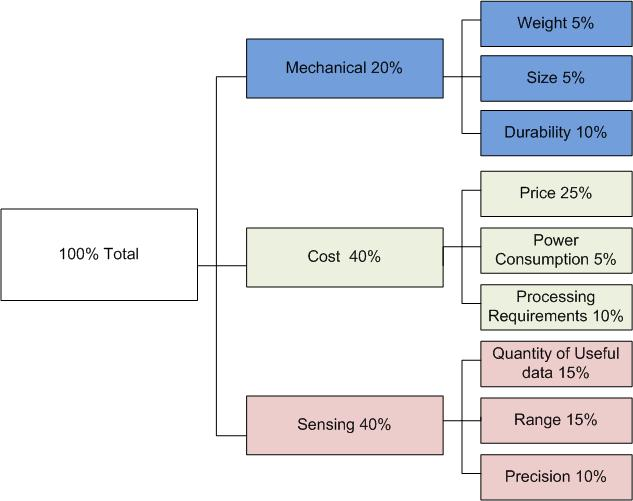
\includegraphics[scale=0.5]{CriteriaWeighting}
 \caption{Criteria Weighting} \label{fig:criteria_weighting}
\end{figure}

\subsection{Weight}
Weight is an important criterion as a number of powered wheel chairs have weight limitations. This should be as small as possible since the weight capacity of a chair like the Invacare Neutron R51LXP is 300 pounds \cite{wheelchair_data}. This means that for any weight we add on to the wheel chair we reduce the potential carrying load of the wheel chair and with it our potential market.

\subsection{Size}
Size is a minor criterion we considered, with an excessively large bulky attachment it would reduce the mobility of the wheel chair and decrease the number of places the wheel chair can travel to. It may also get in the way of the user when operating the wheel chair. This made it important to have some size criteria for measuring the strength of a design.

\subsection{Durability}
While most of the system should not be placed under continuous strain or be at high risk of damage, it is important to consider how durable the design is as there will be wear and tear from use of this system on a wheel chair and damage occurred from movement around the wheel chair.

\subsection{Price}
Price is an important factor for our consideration since we plan to market it to the end users and not to corporations that may have larger budgets. This then made it the most important ranking and with the very large difference in sensor costs it made for a very important factor in determining which route to take.

\subsection{Power Consumption}
Power Consumption measure how much an addition will add to the power consumption of the wheel chair. Many of these chairs are run off of an onboard battery and draining this battery quickly will significantly reduce its usefulness to the users. 

\subsection{Processing Requirements}
The amount of computational intelligence required to handle the data that is coming in from the sensor. This is to make distinction between sensors similar to a Kinect which uses USB and would be plugged into a lab top that will be needed to interpret the data versus something like a sonar sensor that could be tuned and used on FPGA. This will run opposite the Quantity of Useful Data.

\subsection{Quantity of Useful Data}
This was selected to distinguish things like sonar which provide simply a distance mapping for a cone versus something like LIDAR, which provides a high-resolution, narrow-beam distance scan. The more data we get from a sensor the more we can make use of it to recognize and avoid obstacles. This runs as the opposite of processing requirements, since more data requires more processing power to interpret the data.

\subsection{Range}
The range for the detection of objects is fairly important to us. While range beyond 7-8 meters is not particularly useful, we want range from about 0 to 8 meters optimally. For this we assume they are working in optimal conditions which we said to be indoors and with normal lighting. Certain sensors we consider have significantly reduced range in other conditions.

\subsection{Precision}
Precision is fairly important since we are detecting obstacles and we would like to know how far away they are, noise and disturbances are acceptable to a small degree so long as we can identify them as noise and not a fast moving obstacle. In addition to this it is important that some sensors have decreased precision at increased range. This is noted as a small reduction in their score.

\section{Design Review}
Design review was achieved internally through group meetings, collaboration, and testing prior to implementing a final section of the project.

Group members discussed their ideas with one another prior to implementation. When a certain step of the project was considered to be a risk, such as the selection of the final collision avoidance sensors or the design of a custom control PCB, testing was undertaken first to minimize the risk of proceeding. 

Examples of this are testing the Kinect and sonar sensors, which lead to the selection of wide-beam sensors that were controlled individually by our custom PCB to eliminate crosstalk problems between sensors and also confirmation of the Kinect (Primsense) sensor as an excellent design choice (more details in design section). Another example of testing was bread-boarding sections of our custom PCB to control a single direction of the wheelchair (forward/reverse) to prove it worked before implementing the full joystick interface.

Internal review, accomplished through testing and group discussion, lead to excellent quality of the final product. There was no external review for this project other than review of scheduling provided through regular meetings with one of the MTE 482 professors.

\chapter{Electronics and Firmware}

\section{Initial Design}
Electronics and firmware refers to the sections of the project that interface between the wheelchair, the sensors, and the control laptop.

The initial design report discussed that a custom PCB would be designed to manage all of the functions mentioned above. It would be far too messy to wire each sensor individually to the laptop, control the wheelchair through some USB-to-analog box, and then to find power sources for the 12V Kinect sensor and 5V sonar sensors.

The high level design for the control PCB was decided early on and is shown in Figure \ref{fig:hardware_diag}. The PCB would be responsible for powering each of the sensors, controlling the wheelchair (based on laptop commands coming in over USB), and passing user input via joystick/sensor data into a single USB stream to send to the laptop.

\begin{figure}[hbt]
 \centering
 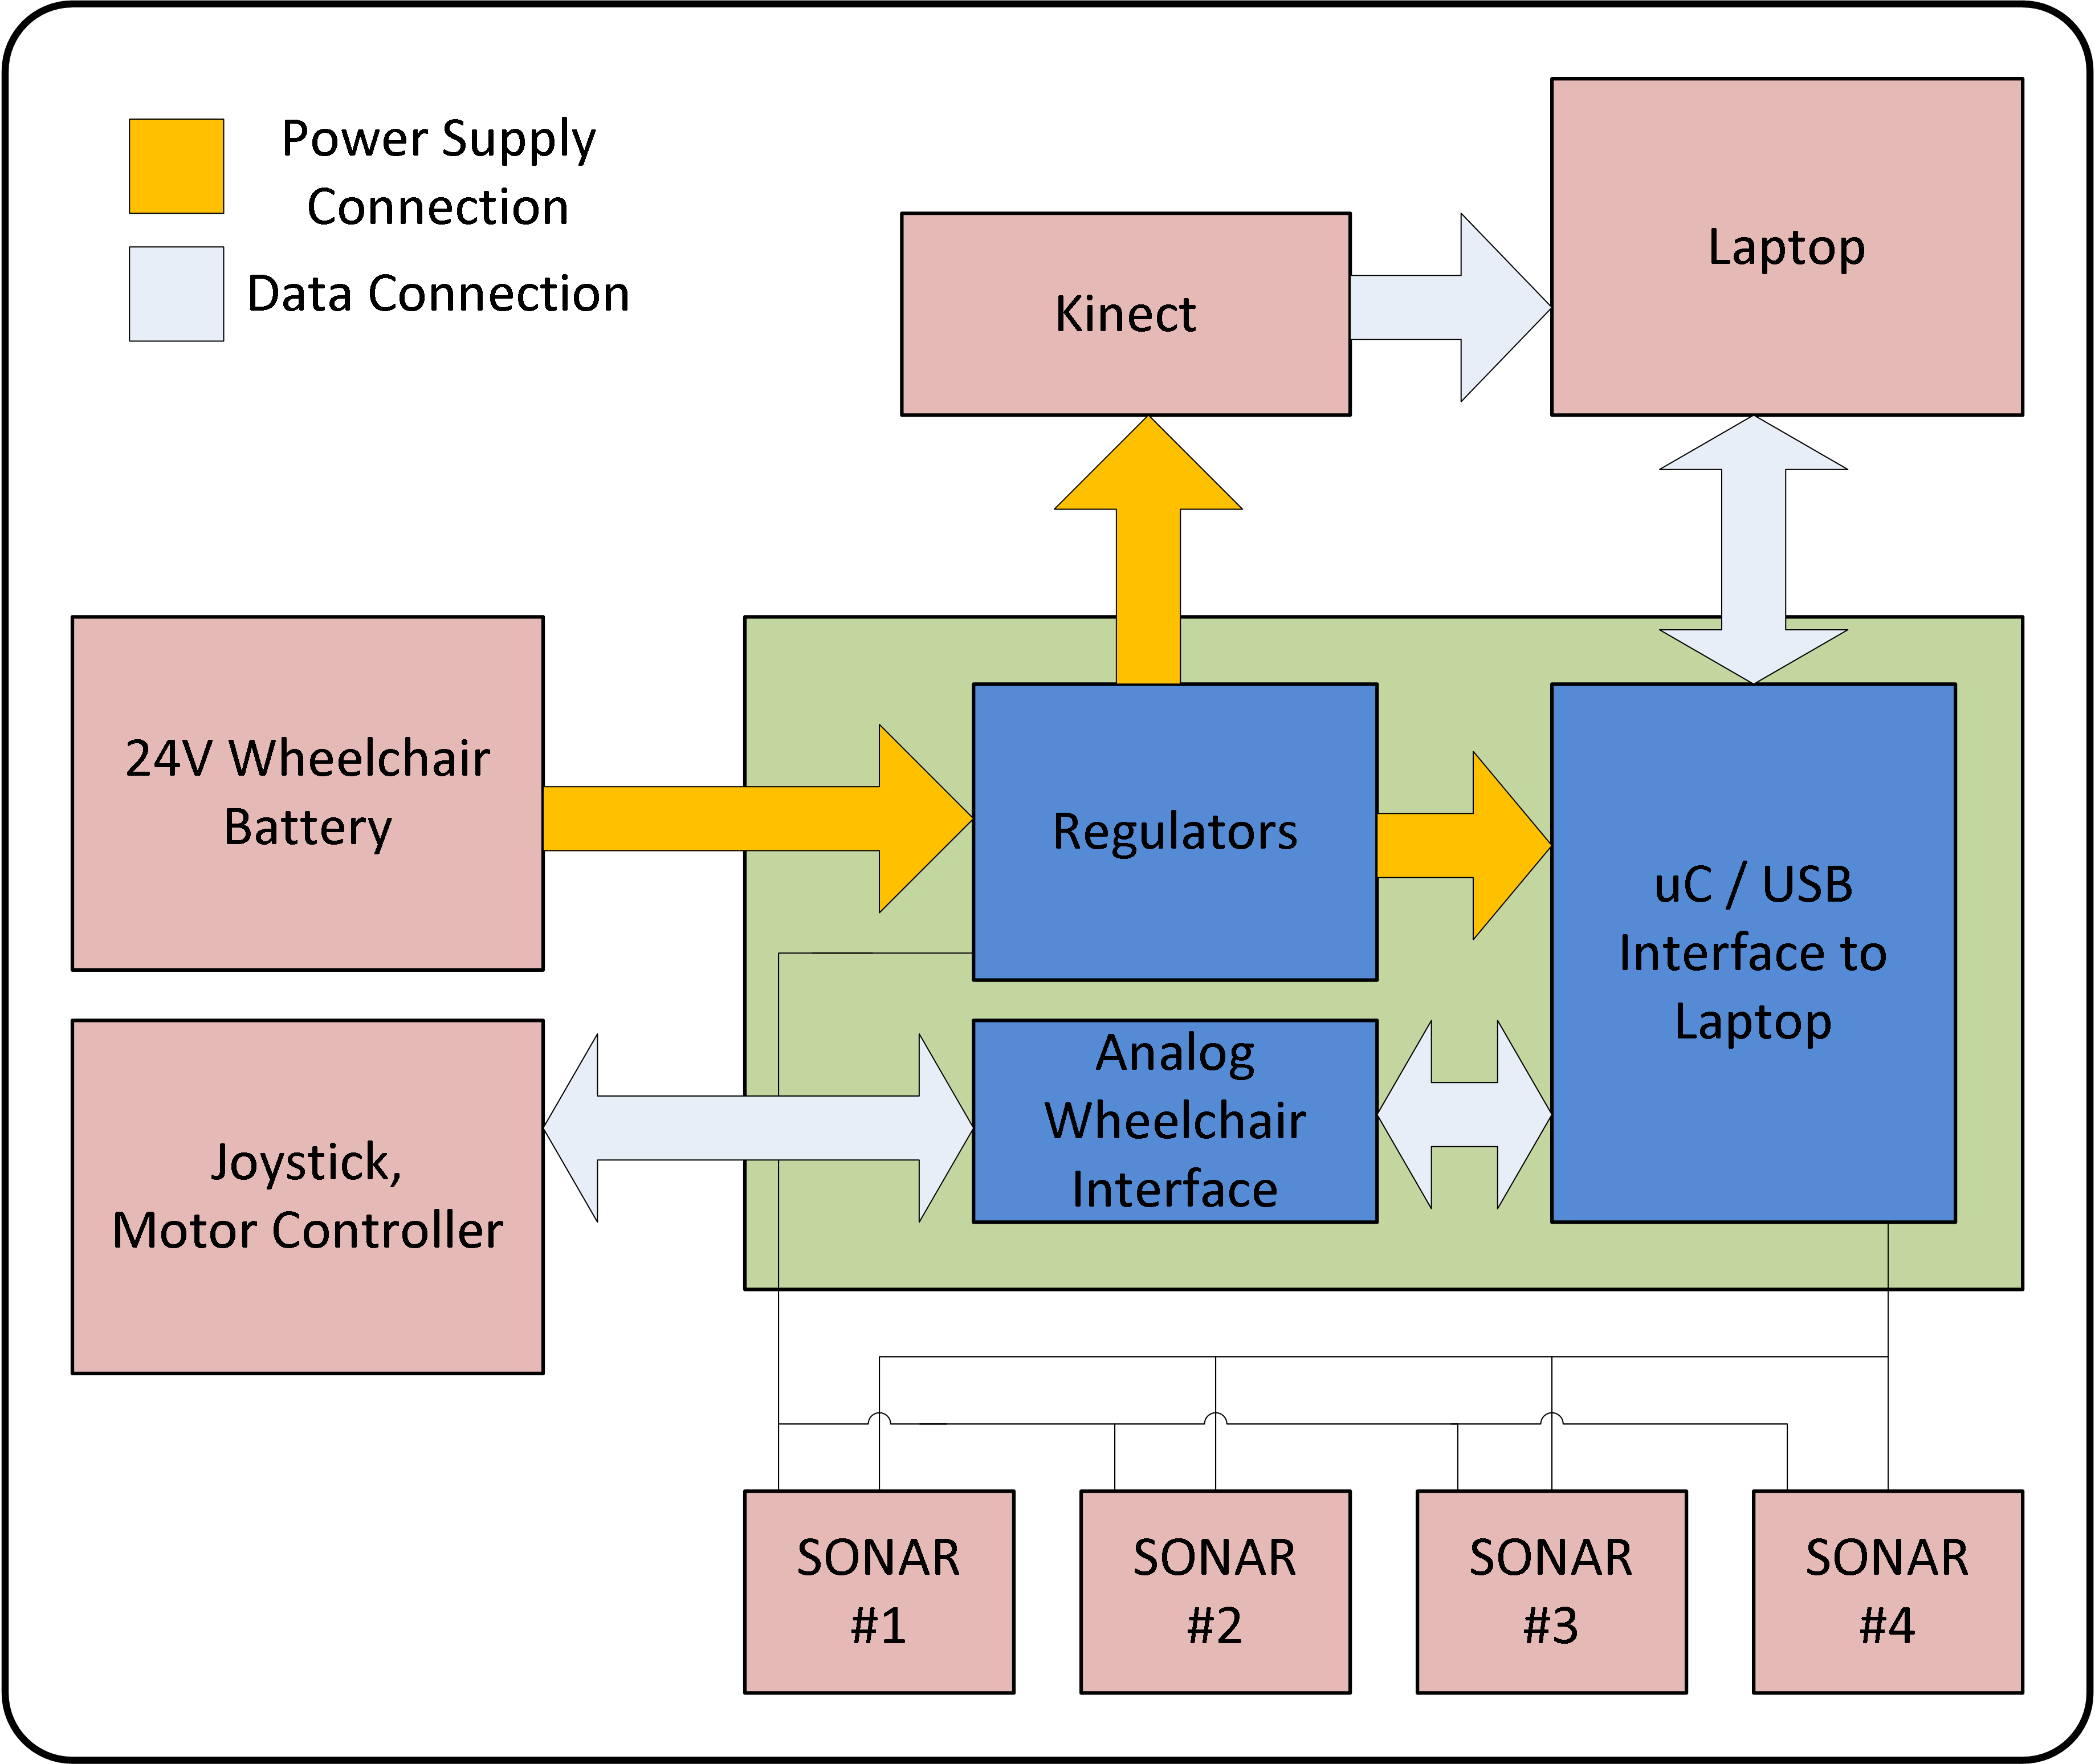
\includegraphics[scale=0.5]{FYDP_PCB_Diagram}
 \caption{PCB Design}\label{fig:hardware_diag}
\end{figure}

In the initial report this was deliberately left at a high level and no detailed schematics were provided. This was due to the problem of controlling the wheelchair and gathering user input via the joystick, the "Analog Wheelchair Interface" section of Figure \ref{fig:hardware_diag}. The joystick module communicates with the motor controllor via a proprietary protocol that is similar to CANbus, but with some small changes. One route we could have taken would be to reverse-engineer the protocol and replace the wheelchair's joystick module entirely with our own PCB and a USB joystick meant for gaming. Our other option was to keep the existing joystick module, and just add a custom PCB and an interposer between the analog signals on the physical joystick and the joystick module PCB that sends serial data to the motor controller. This was as far as discussed in the design report because more testing was needed before we could find the best way to proceed.

\section{Final Design}
The final design filled in all the details that were missing in the initial design. 

The biggest detail was, as mentioned in the previous section, how the wheelchair was going to actually be controlled by the control PCB. To this end, the joystick module was opened up and examined in detail. The joystick was inductively linked to the joystick module's control PCB and the control signals were shown to be sinusoids of approximately 20 kHz. The amplitude of the sine wave increased with as the joystick was moved further from the "home" position, and the phase could be either in-phase with the joystick reference signal (for example in forward/left directions) or 180 degrees out of phase with the reference signal for rear/right stick movement. It was decided this type of control could be relatively easily duplicated on a custom PCB, using a reference sine wave taken from the joystick module and two digital potentiometers (one for each channel) that could modify the amplitude of these waves. By creating a copy of the reference wave and then its inverse and placing these signal at either ends of the digital pots, the signal could be varied from negative full-scale (180 degree phase shift) to DC (joystick home position) to full-scale (in phase with reference signal) in small increments. Also, the existing joystick could be used as an input by using an analog-to-digital converted on our custom PCB and trigging it on the peak of the reference signal input. This saved us the expense of hassle of integrating a USB gaming joystick into the system to allow user control.

Since there was some risk in this control method and by designing a PCB from scratch, a test board was completed as shown in Figure \ref{fig:test_joystick}. This board acted as an interposer between the forward/reverse signals on the physical joystick, and the signals that were sent to the joystick control module. By twisting the analog potentiometer with a screwdriver (the blue component in Figure \ref{fig:test_joystick}) the wheechair was able to be moved forwards and reversed. With this circuit proven out the only risk that was added by a custom PCB was the digital pot versus the analog one, which was really almost no risk at all.
\begin{figure}[hbt]
 \centering
 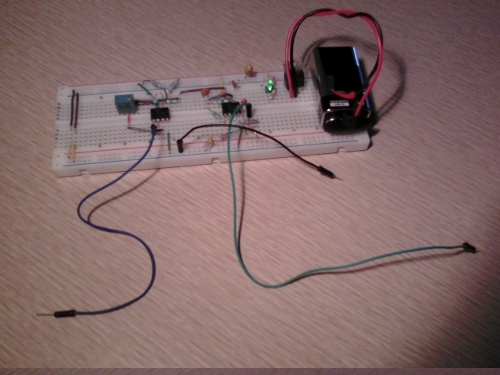
\includegraphics[scale=0.5]{test_circuit}
 \caption{PCB Design}\label{fig:test_joystick}
\end{figure}

With that proven out, the final custom PCB could be designed. Please refer to the Appendix for detailed schematics. The PCB implemented all the high-level features mentioned in the initial report, as well as the analog interface for joystick input and motor controller output just previously mentioned. A CAD model of the PCB as designed is shown in Figure \ref{fig:PCB}.
\begin{figure}[hbt]
 \centering
 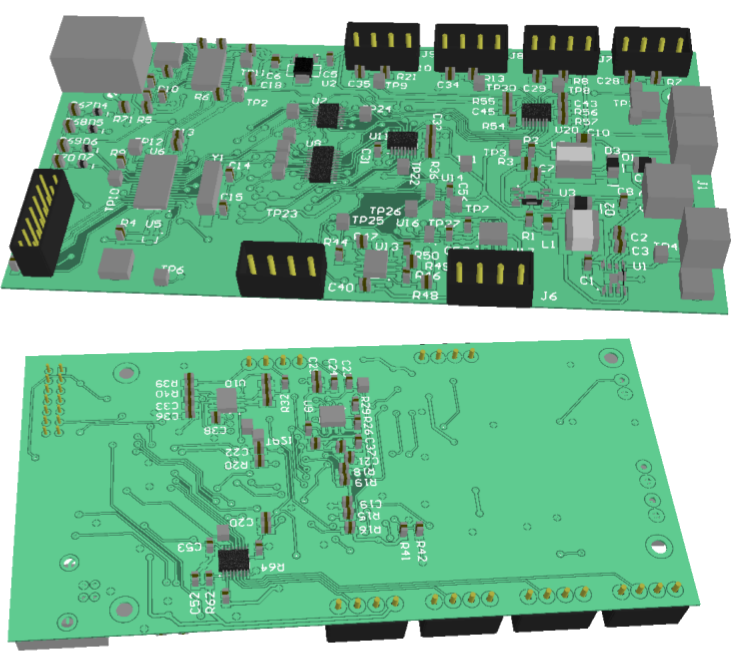
\includegraphics[scale=0.5]{PCB_Custom}
 \caption{PCB CAD Model}\label{fig:PCB}
\end{figure}

The PCB was designed as a 2-layer board and manufactured externally. Once it arrived the components were soldered entirely by group members. There were no major changes that had to made to the PCB after it was manufactured, due in part to the test circuits and proof-of-concepts mentioned previously. A final view of the PCB mounted to the wheelchair and wired is shown in Figure \ref{fig:PCB_wired}.
\begin{figure}[hbt]
 \centering
 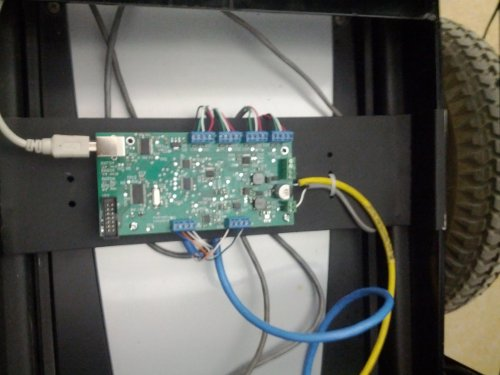
\includegraphics[scale=0.5]{chair_wired}
 \caption{Finished PCB Mounted to Wheelchair}\label{fig:PCB_wired}
\end{figure}

Firmware design was straightforward. The parts selected on the PCB were already familiar to group members and drivers for the digital potentiometers and the analog-to-digital converters was not time consuming. There was some considerable attention spent on the safety of the design: a watchdog timer will trip if the laptop fails to send a command to the PCB every 125 ms, if the PCB firmware itself does not respond every 15 ms, or if a short/open circuit is detected on the user's joystick. Thus in the case of a laptop software, PCB firmware, or joystick wiring fault the wheelchair will come to stop and not risk injury to the user. If there are no errors present the PCB simply relays information to and from the laptop computer.


\chapter{Collision Sensors}

\section{Initial Design}
The initial selection of sensors was to use a Primesense depth sensor in the form of an Xbox Kinect, and 4 sonar sensors, one of each corner of the wheelchair.

Some early testing was done to verify the positioning of the sensor as shown in Figure \ref{fig:testing}. The Kinect position was found to be very good and kept where it is shown in Figure \ref{fig:testing}. Testing showed the sonar sensors should be swapped for wide-beam sensors and angled as shown in Figure \ref{fig:sonar_config}.
\begin{figure}[hbt]
 \centering
 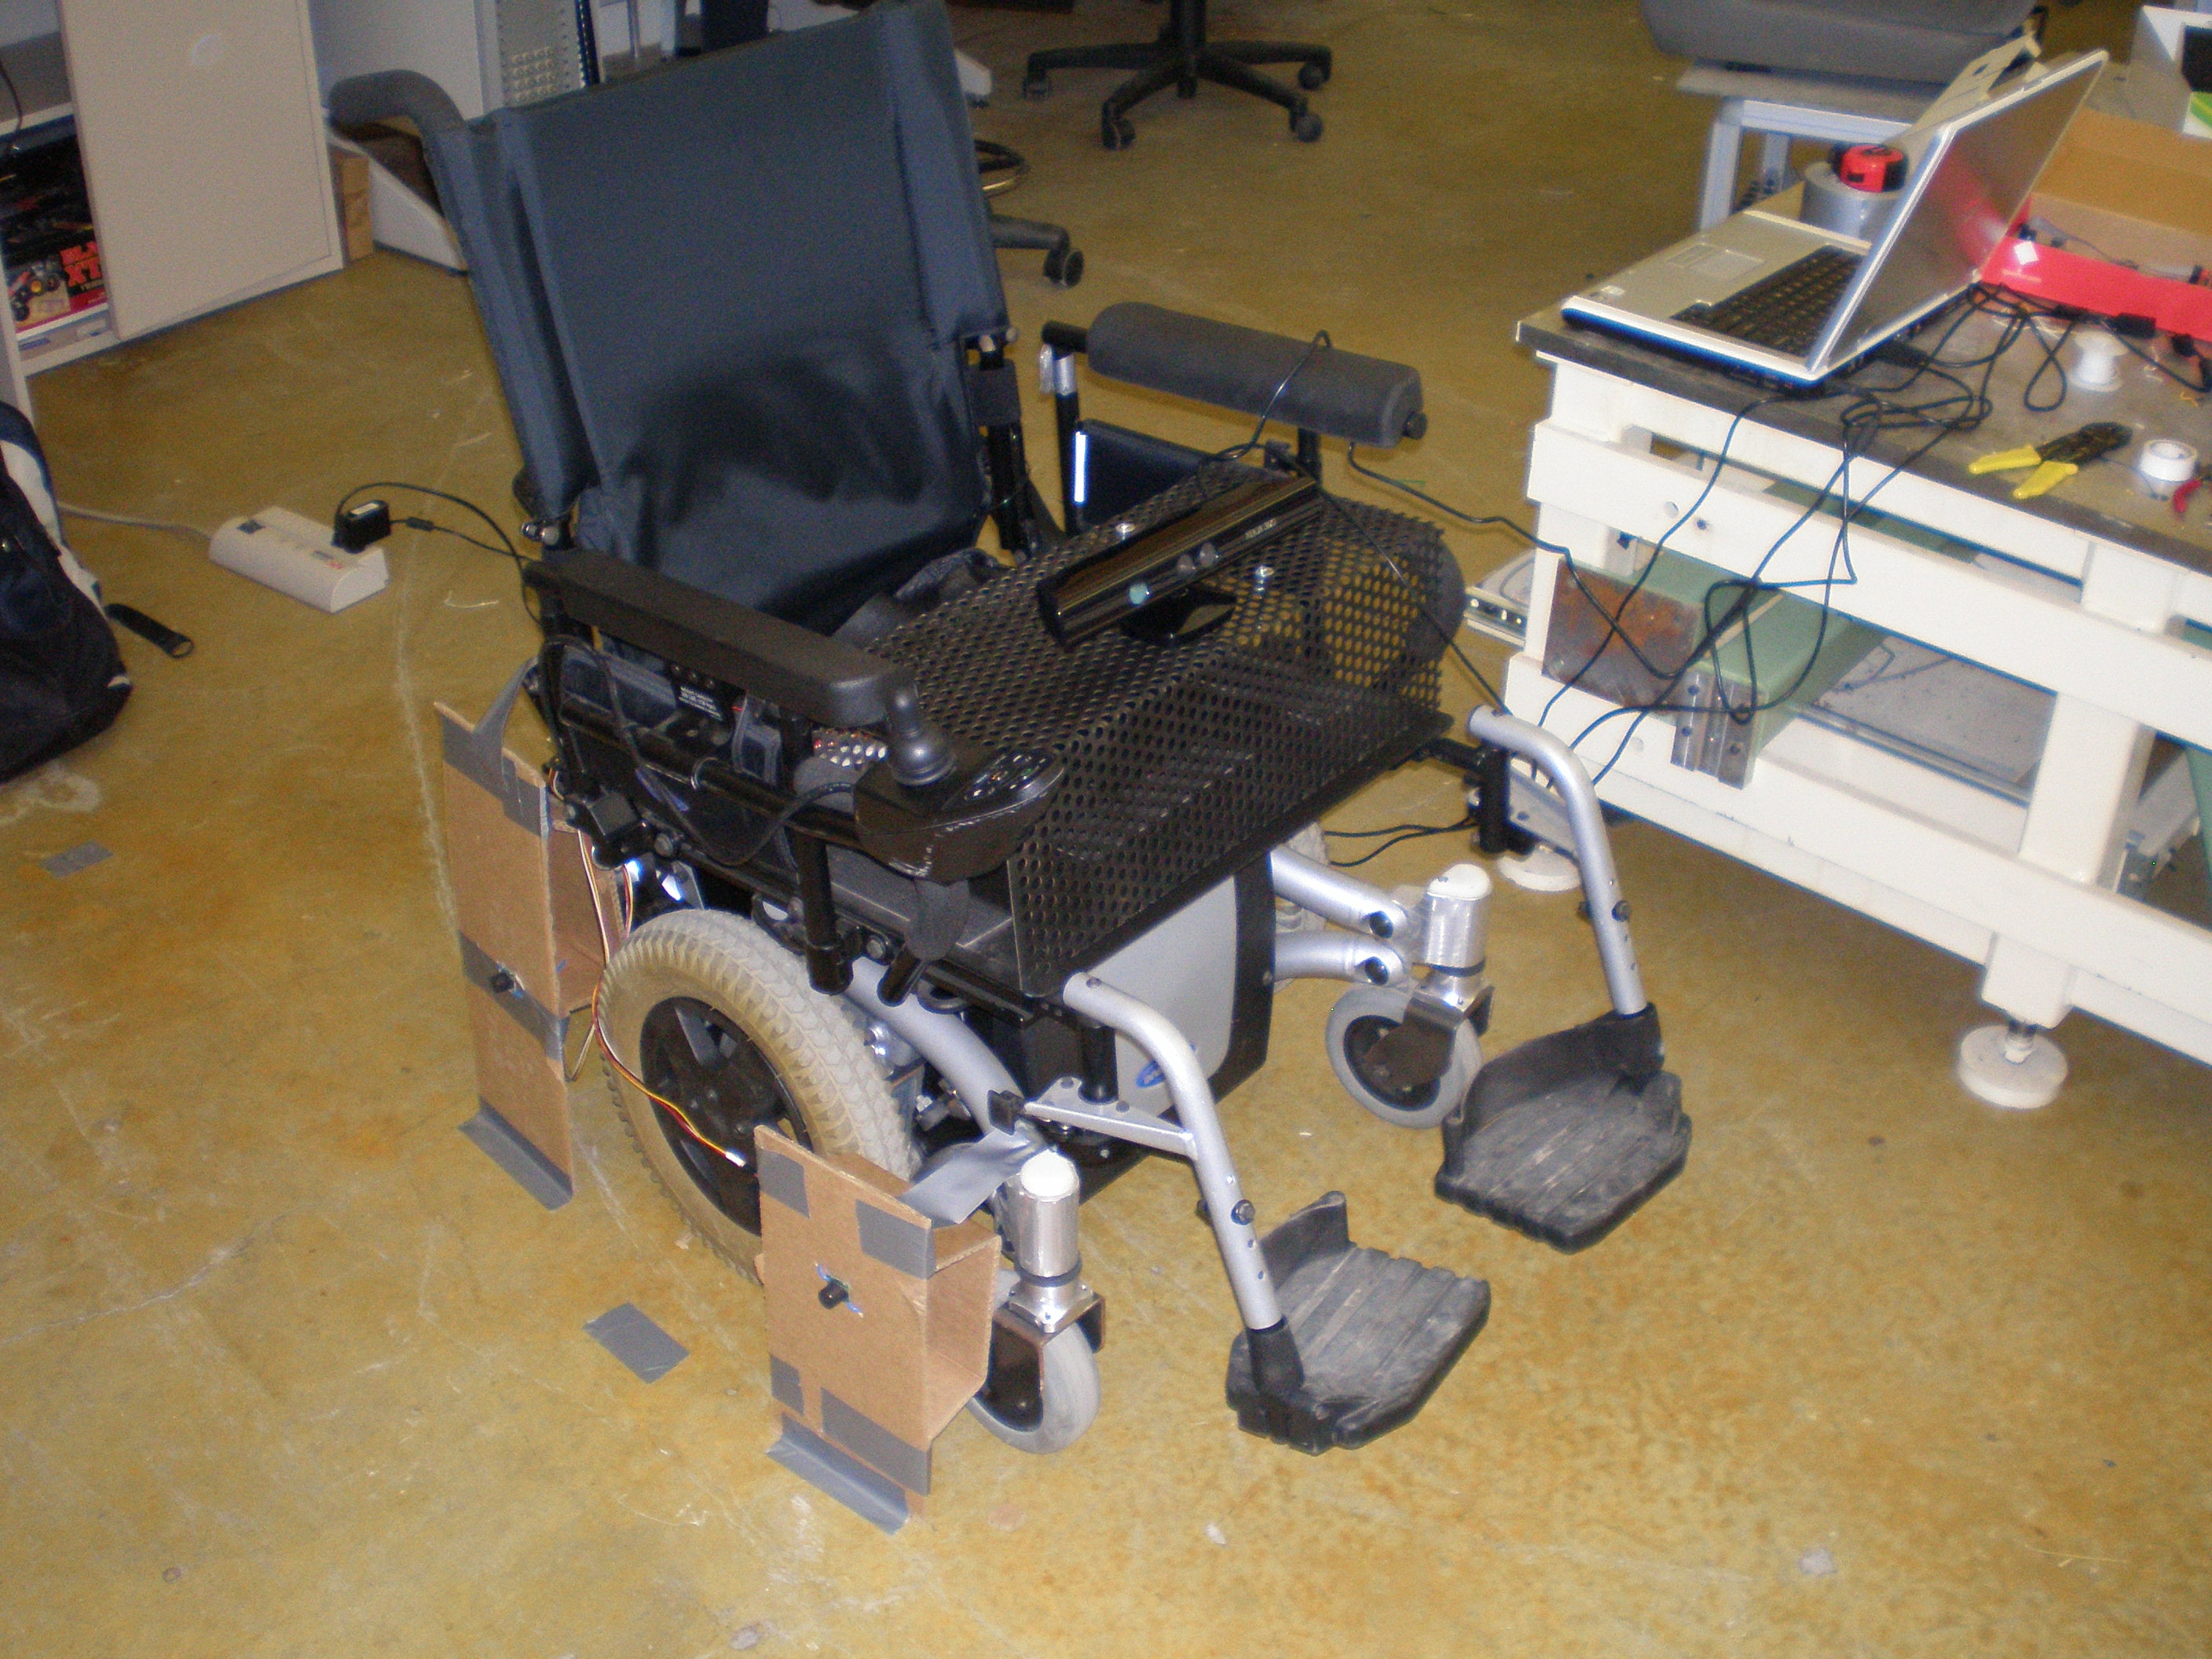
\includegraphics[scale=0.1]{testing}
 \caption{Early Test Setup for Kinect and Sonar Sensors}\label{fig:testing}
\end{figure}
\begin{figure}[hbt]
 \centering
 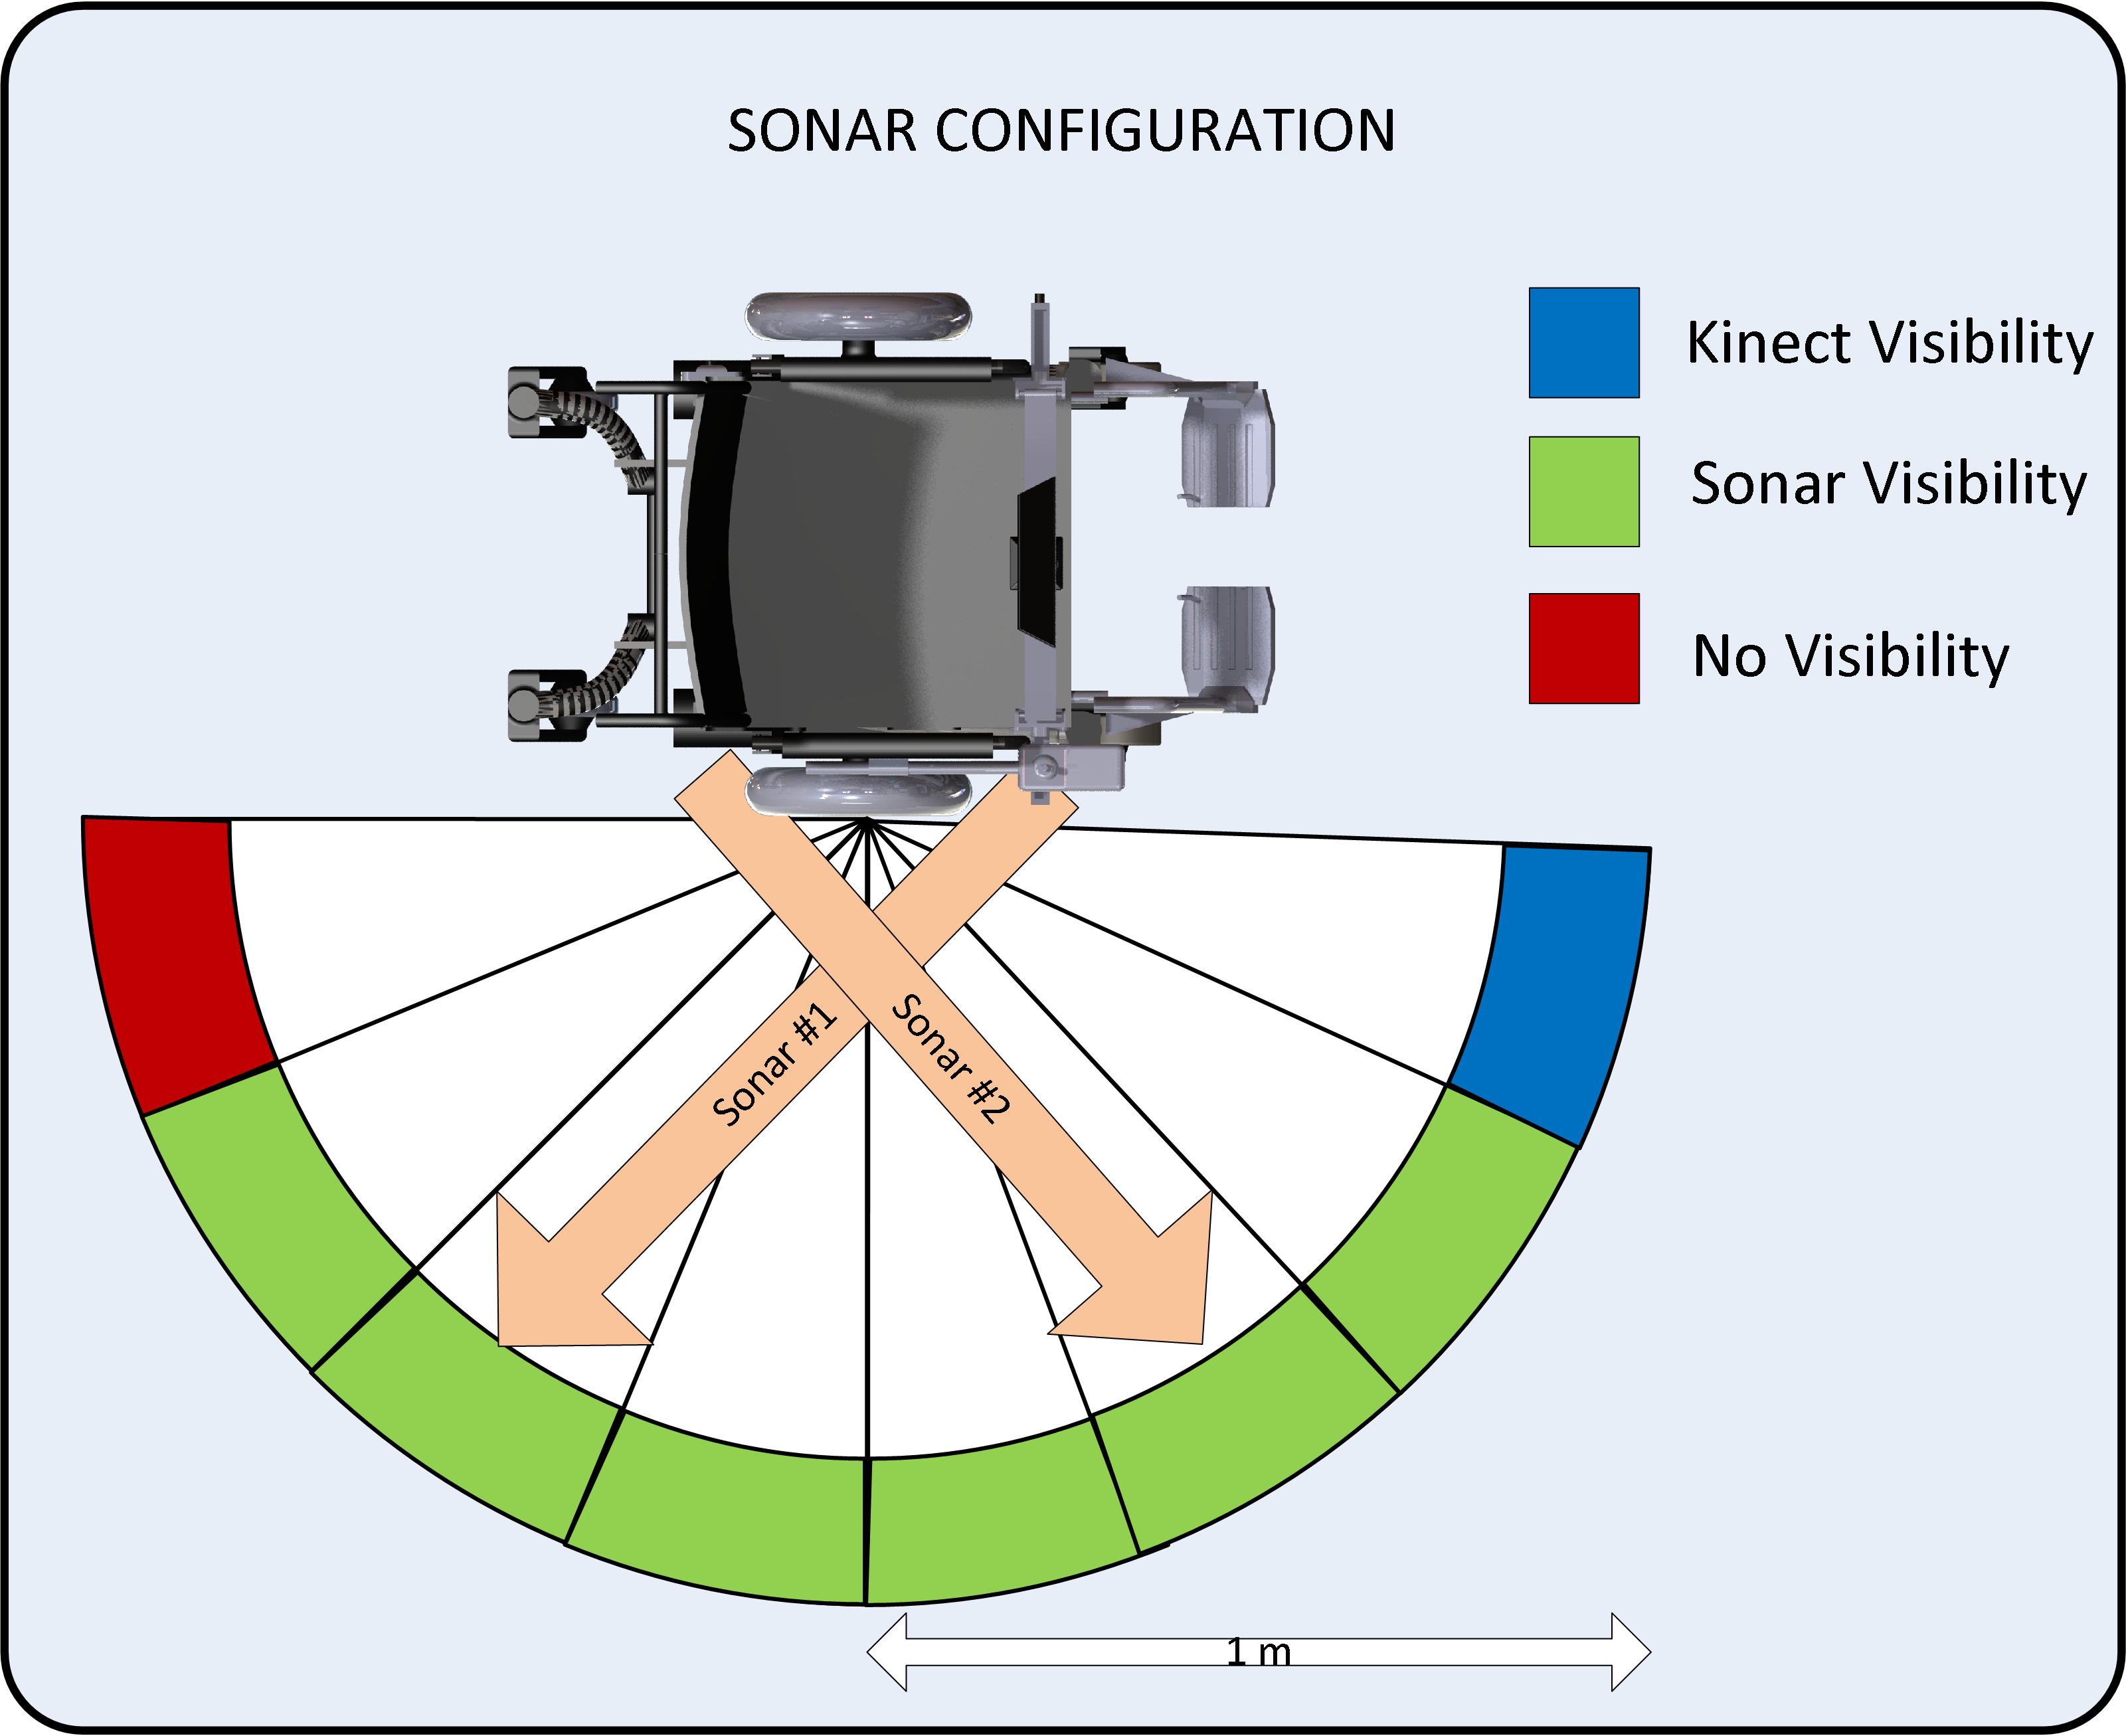
\includegraphics[scale=0.55]{SONAR_Config_Final_Report}
 \caption{Sonar Sensor Configuration}\label{fig:sonar_config}
\end{figure}

\section{Final Design}
The final design implemented the recommendations shown from early testing. The Kinect sensor position was maintained as shown in Figure \ref{fig:testing}, and the sonar sensors were angled as shown in Figure \ref{fig:sonar_config}.

The resulting detectability of obstacles was excellent. The sonars provided a very wide beam width that would alert the wheelchair of any obstacles in the side region of the chair. It was found to work very well for narrow obstacles like table legs as well as wide obstacles such a walls or humans. The Kinect provided very good visibility in front of the wheelchair. Due to its position above the ground there is a small blind spot around the user's feet, but this is solved by not allowing the wheelchair to get within a few feet of an obstacle and proved not to be a large issue.

\chapter{Control Software}

\section{Initial Design}
\begin{figure}[hbt]
 \centering
 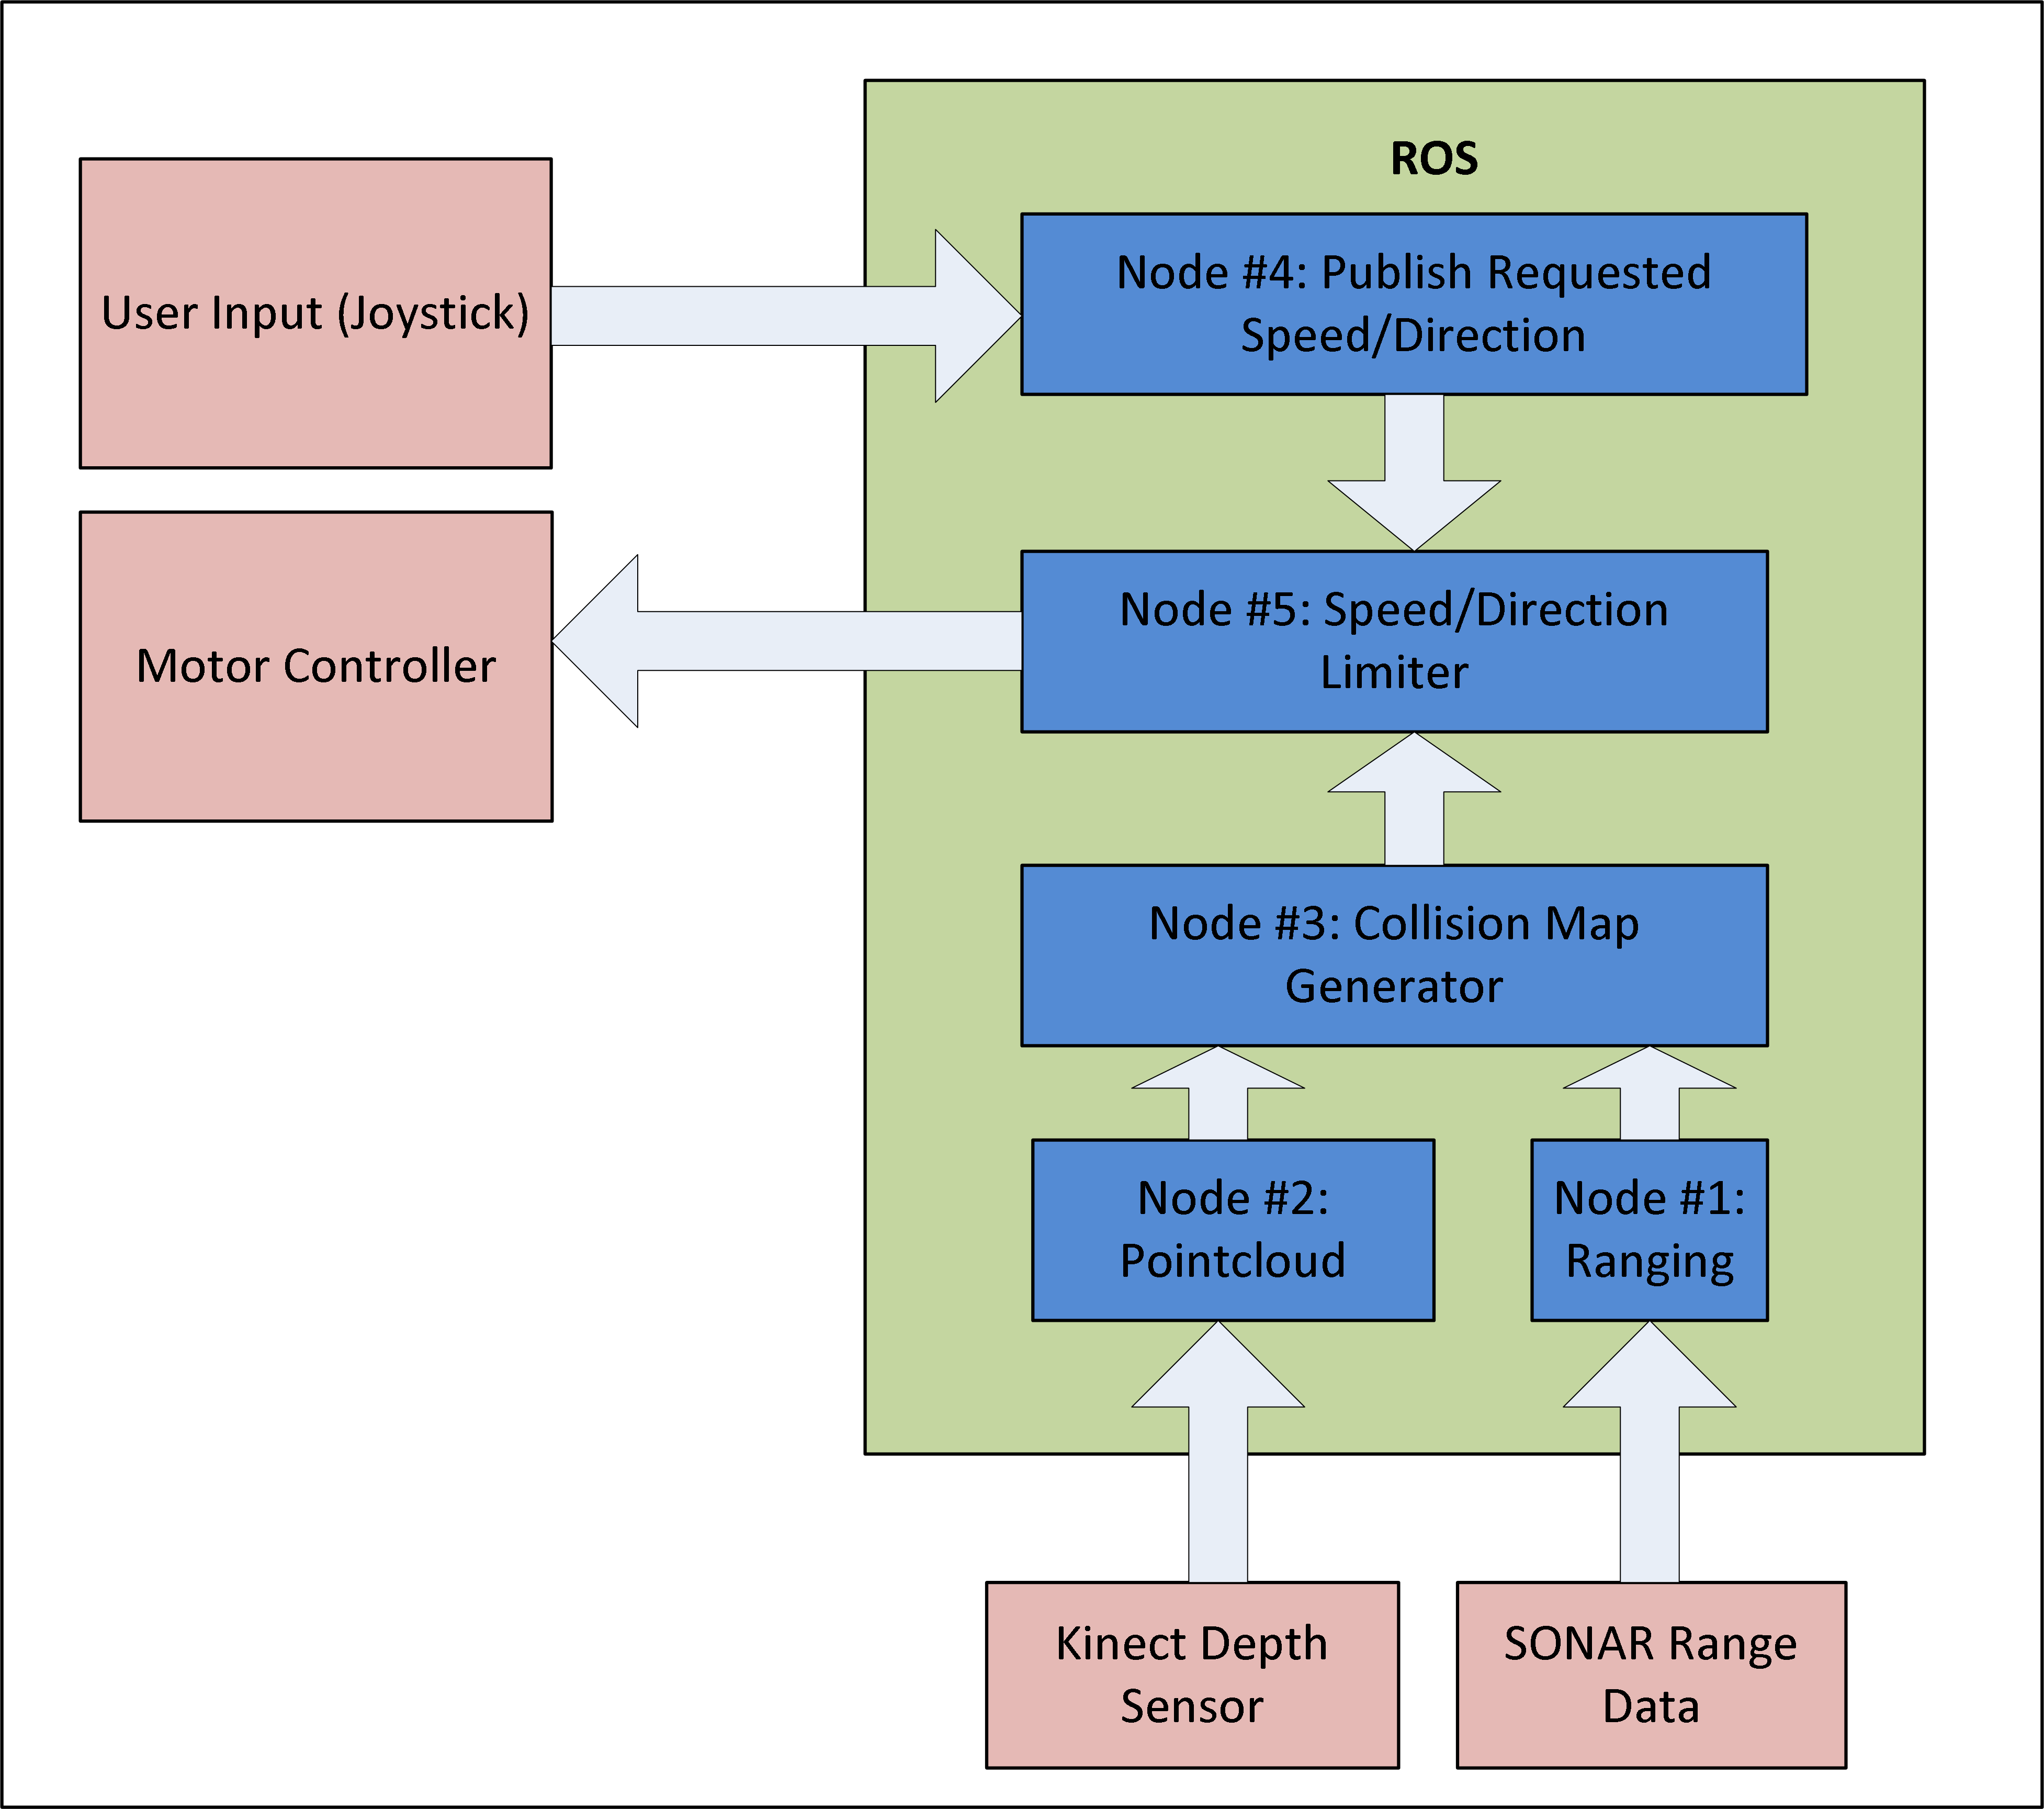
\includegraphics[scale=0.9]{Software_Diagram}
 \caption{Software Design}\label{fig:software}
\end{figure}

Figure \ref{fig:software} shows an overview of the intended software architecture.  Software was intended to be built on the Robot Operating System (ROS) \cite{ROS}, which is a distributed message passing system capable of running on Linux systems.  ROS systems are organized into a network of simple nodes, which co-operate to produce complex aggregate behaviour. 

The following nodes were expected to be required, with the following roles and capabilities:

\subsubsection{Node 1: Ranging}
The ranging node is responsible with communicating with the micro-controller in order to obtain range data from the ultrasonic rangefinders.  It publishes parsed range data.

\subsubsection{Node 2: Point Cloud}
The point cloud node communicates with the Kinect, in order to obtain depth map data.  It publishes point cloud data.

\subsubsection{Node 3: Collision Map Generator}
The collision map generator node is responsible for interpreting poinrt cloud and rangefinder data.  These data are projected into a 2-D occupancy grid in the vehicle frame.  In the simplest case, collision map generation is stateless, and ignores previous data in the interpretation of new sensor data.  If this does not provide sufficient accuracy, the collision map generator might also use state estimates to project old information forward, improving estimates.  

This node subscribes to point cloud and rangefinder data, and publishes collision maps.

\subsubsection{Node 4: Joystick}
The joystick node is responsible for communicating with the joystick, in order to obtain speed and direction commands from the user.  It publishes joystick state.

\subsubsection{Node 5: Speed / Direction Limiter}
The speed / direction limiter node is responsible for communicating with the motor controller in order to set wheel velocities.  It uses a collision map and a wheelchair motion model to assess whether a particular command is likely to lead to a collision.  If necessary, it adjusts user commands in order to avert collisions.

This node subscribes to collision map and joystick command data.  It does not publish anything.

\section{Final Design}
The high-level software architecture has changed substantially since the initial design. Figure \ref{final_arch} shows the block diagram for the implemented system.

\begin{figure}[hbt]
 \centering
 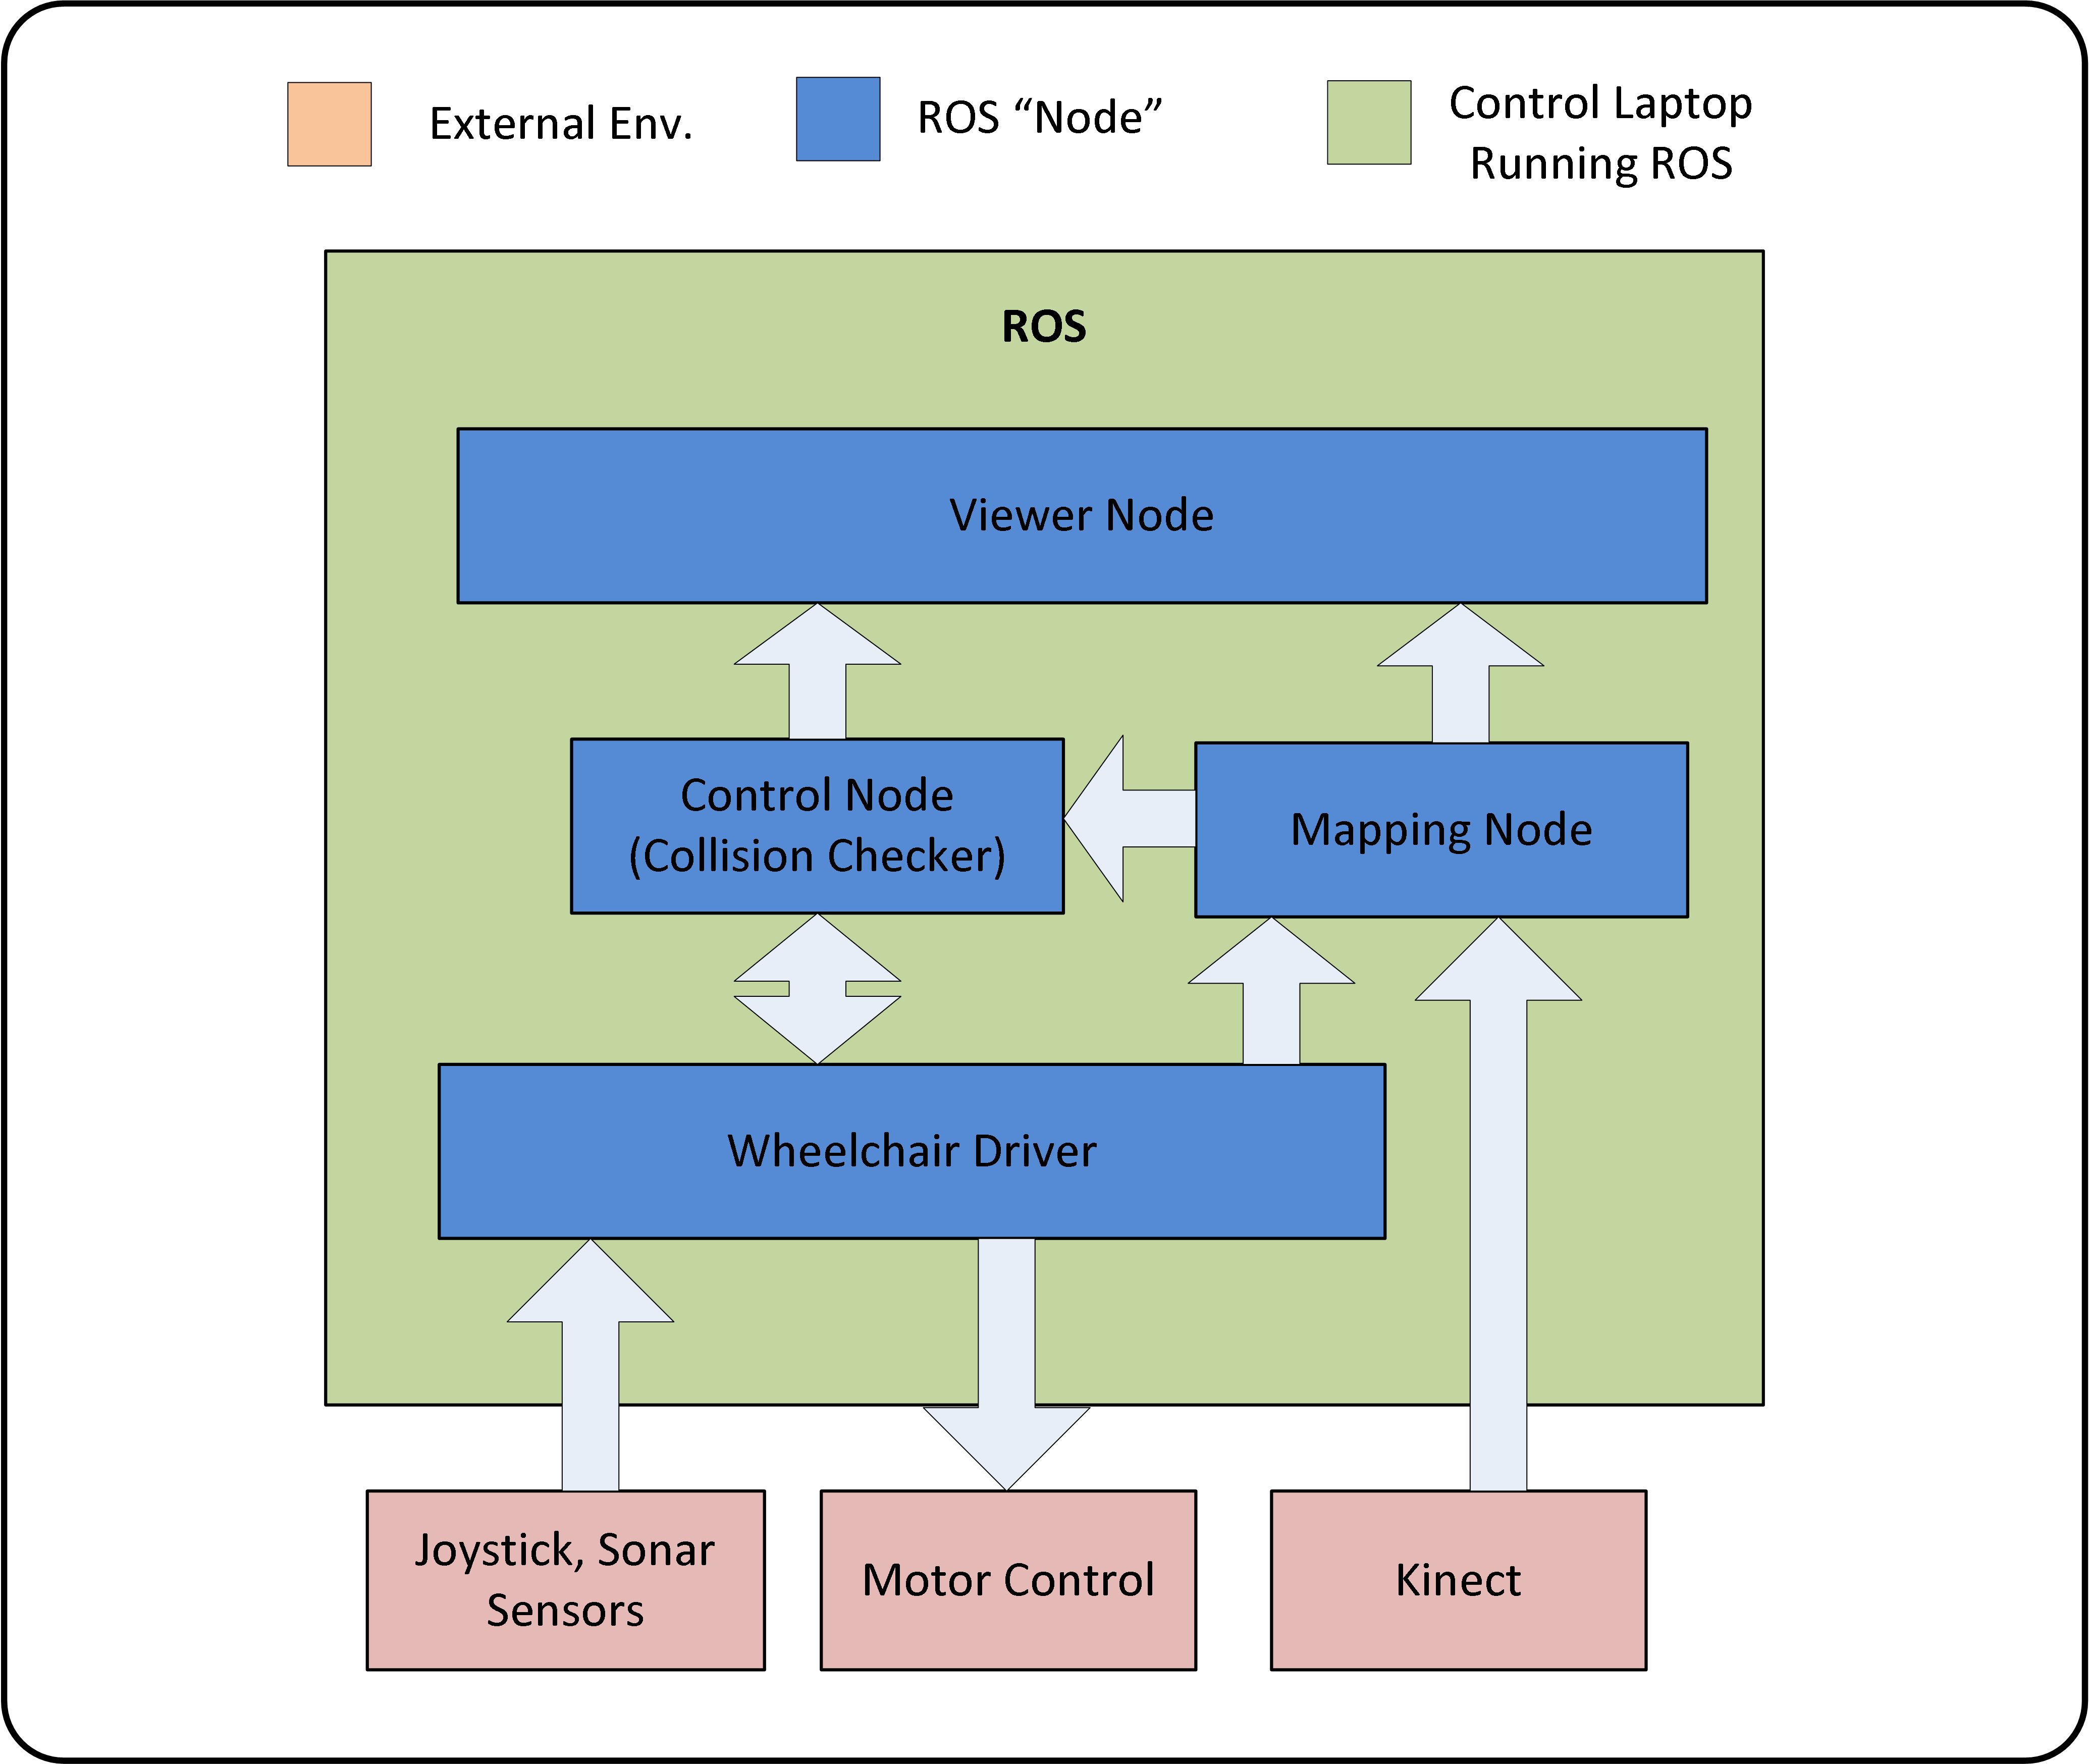
\includegraphics[scale=0.8]{FYDP_Software_Diagram}
 \caption{Final control software architecture}
 \label{final_arch}
\end{figure}


\subsection{ROS Nodes}
The following ROS nodes were included in the final system:

\subsubsection{Wheelchair Driver} 
This node acts as a simple interface between the microcontroller and other ROS nodes.  It has exclusive access to the serial device file associated with the microcontroller, and implements the serial protocol used to send messages to and receive messages from the device.  This node publishes all ranging and joystick input data received from the microcontroller.  It also subscribes to output command messages, which it passes on to the microcontroller.

\subsubsection{Mapping Node} 
This node is responsible for interpreting sensor input in order to produce an occupancy map for the region around the wheelchair.  It subscribes to the sonar range data published by the wheelchair driver, and the pointcloud data published by the off-the-shelf Kinect nodes.  Whenever it receives new data, it computes and publishes a new occupancy grid.

\subsubsection{Control Node}
This node subscribes to the occupancy maps and input commands.  It publishes output commands and trajectory predictions.  It uses a simple model to predict the motion that will result from the input, and checks this path against the occupancy map to predict how soon a collision will occur, if at all.  If the predicted path is safe, the input will be published unmodified as a output command.  If the predicted path is unsafe, the input will be modified in order to prevent collision before being published.

In addition to its normal operation, the control node monitors a parameter value which specifies whether motion is permitted.  If this parameter specifies that motion should be disabled, then the controller node will always publish a zero output.

\subsubsection{Viewer Node}
This node provides a simple user interface for the sytem.  It subscribes to occupancy maps and trajectory predictions.  It uses OpenGL to draw the occupancy map and predicted trajectory, which provides a simple view into the operation of the system.  The viewer node also provides a mechanism for setting the parameter which enables and disables wheelchair motion.

\subsection{Serial Protocol}
Code used to parse the serial protocol is shown in \ref{appendix:serial_parsing}.

The microcontroller and wheelchair driver communicate using a simple, message-based binary protocol.  On the wire, messages have the following structure:

\begin{figure}[hbt]
 \centering
 \begin{tabular}{|l|c|}
  \hline
   Sync Byte 1 & 0xAA \\ \hline
   Sync Byte 2 & 0x55 \\ \hline
   Checksum & 1 byte \\ \hline
   Message Type & 1 byte \\ \hline
   Message Length & 1 byte \\ \hline
   Payload & 0-255 bytes \\ \hline
 \end{tabular}
\end{figure}

The sync bytes are included at the beginning of every message.  Their purpose is to ensure that the microcontroller and wheelchair driver can synchronize if they begin receiving parway through the message, and recover if they lose synchronization due to lost or corrupted data.  The checksum is simply a cumulative XOR combination of all subsequent bytes in the message.  This provides rudimentary error detection capabilities.  The message type indicates to the receiver how the message should be interpreted.  Finally, the message length encodes the length of the payload, which is used in parsing, and is useful for the support of variable-length message types.

\subsection{Occupancy Grid}
Kinect pointcloud data and sonar range data are combined to produce an occupancy grid.  

Computation of the occupancy grid from the point cloud is straightforward.  A particular volume of interest is set, and points outside that volume are ignored.  Points within that volume are projected onto a horizontal plane.  Whichever cell they lie in is set to the `occupied state'.

Code which projects the pointcloud into a 2D plane is shown in \ref{appendix:pointcloud_flatten}

It is also fairly simple to obtain an occupancy grid from rangefinder data.  The rangefinders have a wide field of view, so there is significant ambiguity as to the specific location of the object detected by the rangefinder.  In order to represent this, an arc is drawn in the occupancy map, covering the full field of view of the sensor.

Code which draws rangefinder argcs is shown in \ref{appendix:range_occupancy}.

The occupancy maps computed from pointcloud and rangefinder data are then merged using an elementwise logical OR.

\subsection{Trajectory Prediction}
\label{section:trajectory_prediction}
See \ref{appendix:trajectory_prediction} for path prediction code.

The trajectory of the wheelchair is predicted using an extremely simplistic motion model, where the forward velocity and angular velocity are taken to be related to the input command by constant coefficients.  This model is described by the following equations:

\begin{equation}
x_t = x_{t-1} + \Delta T K_f u_f \cos (\theta_{t-1})
\end{equation}
\begin{equation}
y_t = y_{t-1} + \Delta T K_f u_f \sin (\theta_{t-1})
\end{equation}
\begin{equation}
\theta_t = \theta_{t-1} + K_{\theta} u_{\theta}
\end{equation}
Where $K_f$ and $K_\theta$ are empirical constants, and $u_f$ and $u_\theta$ are the forward and lateral inputs supplied by the joystick, respectively.

\subsection{Collision Detection}
\label{section:collision_detection}
See \ref{appendix:collision_detection} for collision detection code.

Primarily, collision detection is accomplished by checking whether the centrepoint any occupied occupancy grid cells fall within a convex bounding polygon for the wheelchair.  Each of the discrete pose samples along the projected path is tested for collision in this manner.

This collision detection technique is built on the use of intersection of half spaces to test whether a convex polygon contains a point.  Figure \ref{fig:point-in-poly} should help to illustrate how this technique works.

\begin{figure}
 \centering
 \includegraphics[scale=0.9]{point-in-poly}
 \caption{Illustration of point-in-polygon testing}
 \label{fig:point-in-poly}
\end{figure}

Given a polygon with $M$ vertices, under the assumption that the polygon is convex and planar, and that all points lie in the plane of the polygon, a given point $Q$ is continaed by the polygon iff 
\begin{equation}
 (Q-P_i) \cdot B_{i,i+1} \ge 0 \quad \forall i = 1, 2, \cdots M-1
\end{equation}
Where $B_{i,i+1}$ is the binormal along the segment from $P_i$ to $P_{i+1}$, which is defined as
\begin{equation}
 B_{i,i+1} = N \times (P_{i+1} - P_{i})
\end{equation}
Where $N$ is normal to the plane of the polygon.

\subsubsection{Use of Rangefinders}
Initially, it had been intended that range data would be used to populate the occupancy grid, and that only the above technique would be used to detect collisions.  

Unfortunately, it was found that the occupancy grid did not have sufficiently high resolution to adequately detect potential collisions with obstacles which are close to the sides of the wheelchair.  As a consequence, range measurements are used independently from the occupancy grid to detect such obstacles, and to restrict rotation in these situations.

\subsection{Control Law}
See \ref{appendix:control_law} for code implmenting the control law.

The intent of the controller is to enforce a lower bound on the time to collision.  

The time to collision is estimated using the techniques described in \ref{section:trajectory_prediction} and \ref{section:collision_detection}.  Using the simple motion model described in \ref{section:trajectory_prediction}, a simple open-loop controller for time to intersect may be derived:

\begin{equation}
u_f^* = \frac{T_{target}}{T_{predicted}(u_f, u_\theta)} u_f
\end{equation}
\begin{equation}
u_\theta^* = \frac{T_{target}}{T_{predicted}(u_f, u_\theta)} u_\theta
\end{equation}

Where $u_f$ and $u_\theta$ are the inputs supplied by the user, and $u_f^*$ and $u_\theta^*$ are the adjusted inputs supplied to the motor controller.  This control law is applied only if $T_{predicted} < T_{target}$.

\subsubsection{Use of Rangefinders}
To handle objects close to the sides of the wheelchair, a similar control law was applied for the lateral input alone:

\begin{equation}
u_\theta^* = \frac{T_{target}}{T_{predicted}(u_\theta)} u_\theta
\end{equation}

This special-case control law is applied prior to path prediction and application of the first control law.

\section{Potential Improvements}
The current control software implementation is fairly simplistic, leaving room for a number of potentially significant improvements.

\subsection{More efficient Collision Detection}
The collision detection method described in \ref{section:collision_detection} is simple and brute-force.  Rather than testing every occupied cell for membership in a relatively small bounding polygon, a polygon-fill algorithm should be implemented to test whether any of the cells contained within the polygon are occupied.  In addition to requiring fewer computations, this would also make it simple to test whether any part of the cell is contained in the polygon, which would provide a more conservative test than the current method, which simply samples the centrepoint.

\subsection{Navigation Assistance}
The current control law simply restricts input to prevent collision, providing no assistance for navigation around obstacles.  This can be somewhat annoying in tight quarters, where predictions based on instantaneous input show collisions, making it difficult to navigate complex paths.  

In these circumstances, it may be helpful to attempt to plan a collision free path which approximately follows the user input commands.  A simple potential field path planner may be sufficient for this purpose.  Alternatively, a rapidly expanding random tree might be expected to provide good results.   

\subsection{Advanced Mapping}
The current mapping technique is simple and stateless, discarding old information whenever new information becomes available.  Although this works reasonably well, improved mapping techniques could lead to significant performance improvements.  

Currently, if an obstacle moves out of the field of view of the sensors, it is quickly forgotten.  This is a significant weakness, as it leads the system to fail to avoid collisions with low-lying obstacles.

The Kinect sensor incorporated in this design provides more than sufficient data for a VSLAM approach \cite{kinect_vslam}.  In fact, an implementation of this approach is already available for ROS.  This would allow the wheelchair to build a detailed map and locate itself in a fixed co-ordinate system as it moves, which would allow the system to avoid previously observed obstacles which are outside the current field of view, and would also allow for more effective path planning.

\chapter{Mechanical}

\section{Initial Design}

\section{Final Design}


\chapter{Project Results}

\section{Prototype Construction}

\section{Testing and Performance}

\chapter{Schedule and Budgeting}

\section{Planned Schedule}
\begin{figure}
 \centering
 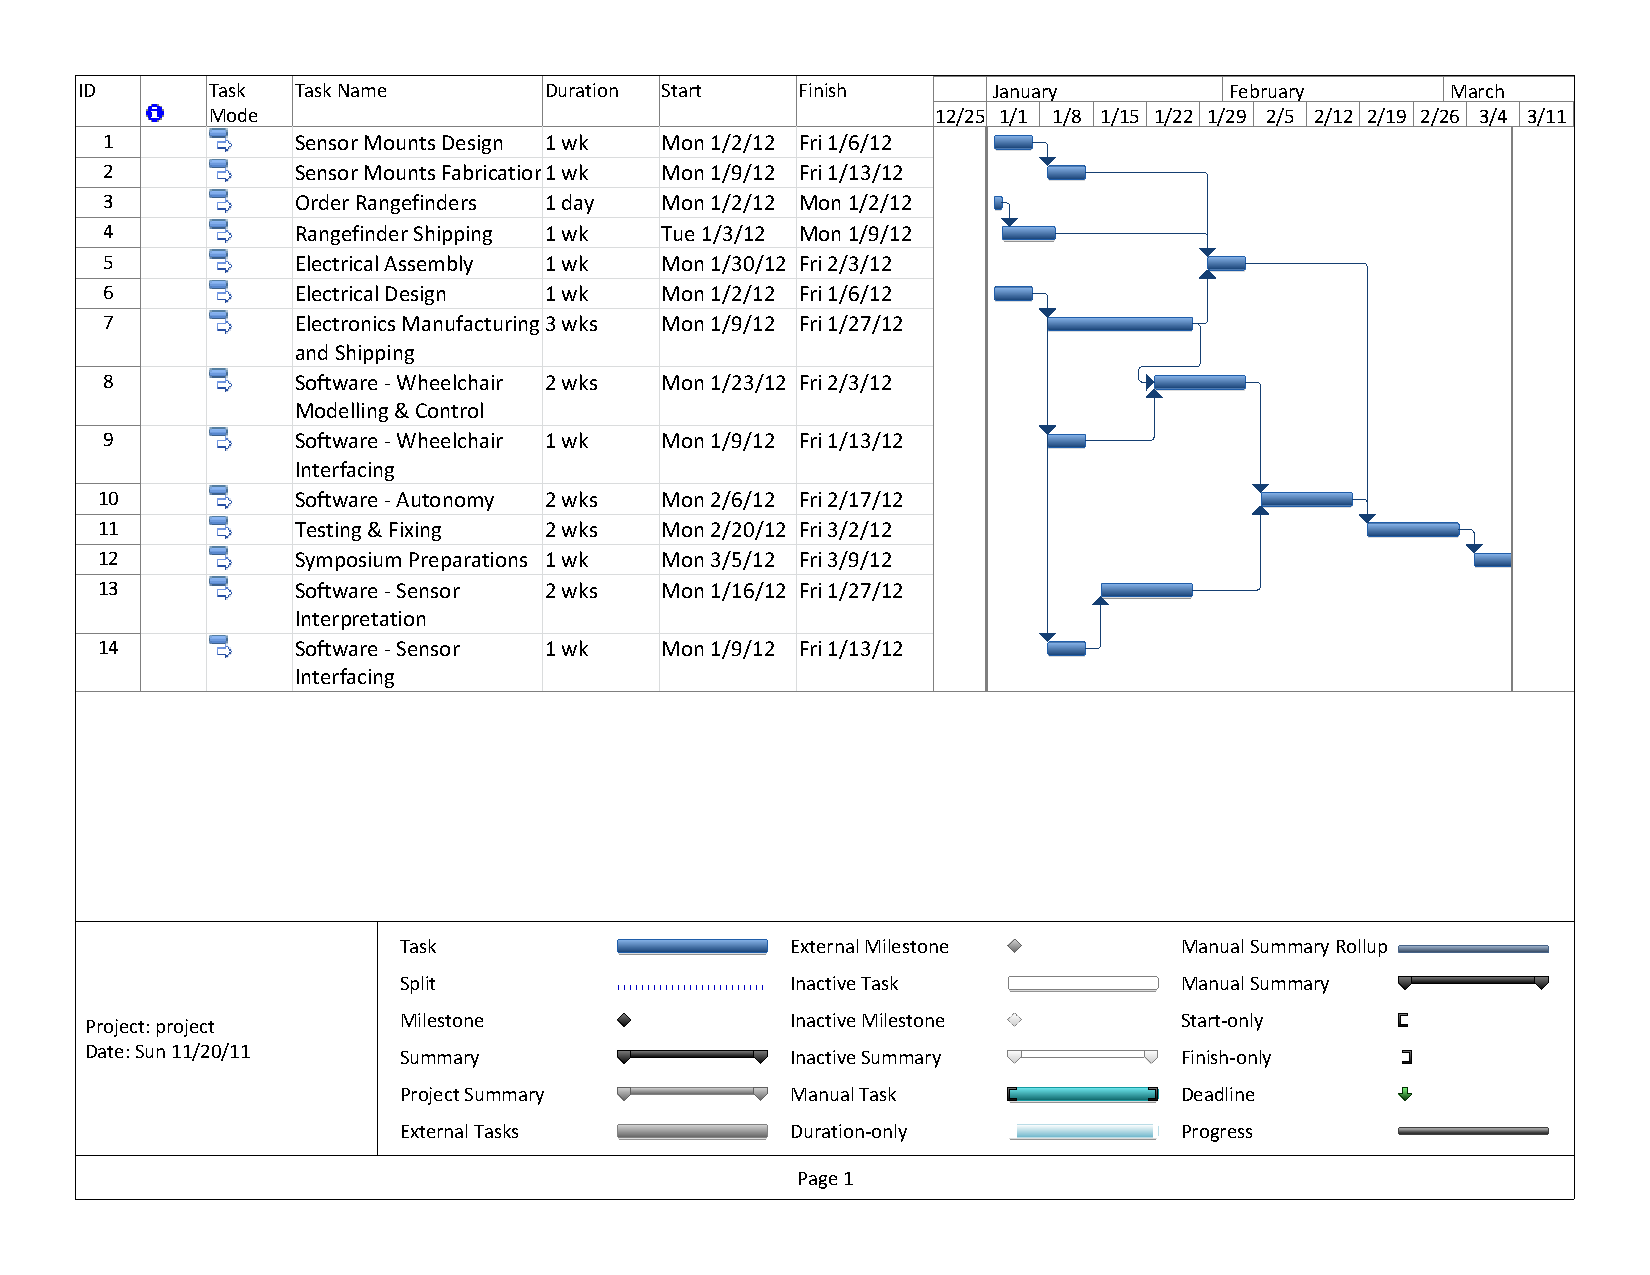
\includegraphics[scale=0.6]{gantt} \label{fig:gantt}
\end{figure}

The planned schedule, as included in the last report, is shown above. We will compare this schedule to the one we tracked for our final project.

\section{Updated Schedule}
\begin{figure}
 \centering
 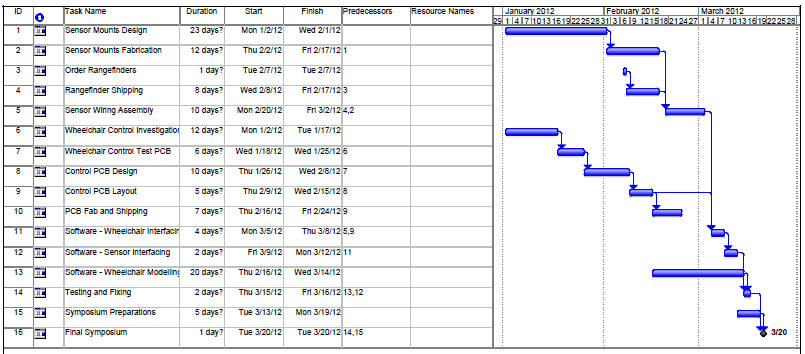
\includegraphics[scale=0.55]{Final_Schedule} \label{fig:final_schel}
\end{figure}

This is the schedule we tracked on our way to the final design symposium. The start dates were slightly delayed versus the planned dates due to extra tasks (external to the project) that tooks group members' time early the term. The schedule was followed closely enough to allow for the project to be delivered early, ahead of schedule. As shown in the chart this lead to a week of testing and improvement. The extra testing time was critical to producing a good demonstration and poster for the symposium that lead to a tie for second-place overall position in the design symposium.

\section{Budget}
The total cost for the BOM for a single collision-avoidance system has been updated from the previous estimate to be as shown in Figure \ref{fig:BOM_single}.

\begin{figure}[hbt]
 \centering
 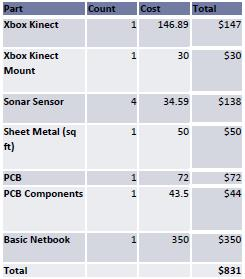
\includegraphics[scale=0.8]{BOM_single}
 \caption{BOM Cost for a Single Unit}
 \label{fig:BOM_single}
\end{figure}

If you recall from the earlier report, it was estimated that approximately \$500 CAD would be an acceptable cost for a collision-avoidance system (based on consultation with industry members). The BOM shown in Figure \ref{fig:BOM_single} exceeds this cost, but a good portion of the prices shown are non-recurring expenses such as setup for the PCB, shipping and handling fees for the electrical components, and the price of the laptop computer required. Figure \ref{fig:BOM_prod} shows  projected BOM costs for production. Here the laptop has been replaced with a single-board computer (the quoted price of \$35 could be for a Rasberry Pi device, for example), and the PCB costs have been slashed to an estimate of unit cost since the non-recurring engineering feels like tooling and setup can be averaged over 100 or more PCBs.

\begin{figure}[hbt]
 \centering
 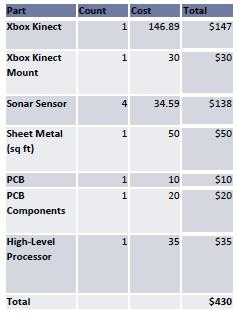
\includegraphics[scale=0.8]{BOM_production}
 \caption{Production BOM Cost Estimate}
 \label{fig:BOM_prod}
\end{figure}

This `production' BOM shown in Figure \ref{fig:BOM_prod} comes in under the \$500 CAD cost that we had targeted as a final BOM expense from the beginning.


\section{Actual Cost}

A listing of the actual cost of this project is shown in Figure \ref{fig:costs}. No laptop is included as group members' computers were used for the project symposium. Two PCBs were manufactured as a backup so costs are higher than shown in Figure \ref{fig:BOM_single} in the BOM costs for a single unit. Extra shipping duties included in Figure \ref{fig:costs} were not included in the BOM cost calculations of the previous section.

\begin{figure}[hbt]
 \centering
 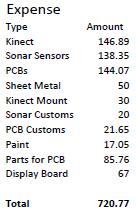
\includegraphics[scale=1]{Project_Expenses}
 \caption{Project Expenses (CAD)}
 \label{fig:costs}
\end{figure}


\chapter{Conclusions and Recommendations}

% Set special section numbering for appendices
\renewcommand{\thesection}{\Alph{chapter}.\arabic{section}}

\chapter*{Appendix A - Selected Control Software Code Listings}
\setcounter{chapter}{1}
\addcontentsline{toc}{chapter}{Appendix A - Selected Code Listings}
Complete source code can be obtained at http://github.com/ipeet/mte481

\section{Serial Protocol Parsing State Machine}
Excerpt from common/serial/protocol.c
\label{appendix:serial_parsing}
\begin{lstlisting}
 // Parse a new byte
enum ParseStatus pr_push(uint8_t byte) {
  if (_state == DONE) {
    // start reading a new message
    pr_init();
  }

  switch (_state) {
    case SYNC_1:
      if (byte == SYNC_BYTE_1) {
        _state = SYNC_2;
        return OK;
      } else {
        return BAD_SYNC;
      }

    case SYNC_2:
      if (byte == SYNC_BYTE_2) {
        _state = CHECKSUM;
        return OK;
      } else {
        pr_init();
        return BAD_SYNC;
      }

    case CHECKSUM:
      _buf.checksum = byte;
      _state = TYPE;
      return OK;

    case TYPE:
      _buf.type = byte;
      _state = LENGTH;
      return OK;

    case LENGTH:
      _buf.length = byte;
      if (byte == 0) {
        _state = DONE;
        break;
      } else {
        _payloadBytes = 0;
        _state = PAYLOAD;
        return OK;
      }

    case PAYLOAD:
      _buf.raw[_payloadBytes] = byte;
      _payloadBytes++;
      if (_payloadBytes < _buf.length) {
        return OK;
      } else {
        _state = DONE;
        break;
      }
    
    default:
      pr_init();
      return INVALID;
  };

  // Should only fall through for checksum on a complete package
  if (_state != DONE) return INVALID;

  /* Validate checksum */
  if (pr_checksum(&_buf) == _buf.checksum) {
    return COMPLETE;
  } else {
    return BAD_CHECKSUM;
  }
}
\end{lstlisting}

\clearpage
\section{Projection of a Pointcloud Into an Occupancy Grid}
Excerpt from wheelchair\_ros/src/occupancy.cpp
\label{appendix:pointcloud_flatten}
\begin{lstlisting}
void Occupancy::handlePointcloud(const PointCloud::ConstPtr &msg) {
  /* Convenience */
  int w = m_width / m_resolution;
  int d = m_depth / m_resolution;
  int h = m_height / m_resolution;

  m_kinect2d.clear();
  m_kinect2d.resize(w*d);

  m_kinect3d.clear();
  m_kinect3d.resize(w*d*h);

  for (unsigned i=0; i < msg->points.size(); ++i) {
    double x = msg->points.at(i).x;
    double y = -msg->points.at(i).y;
    double z = msg->points.at(i).z;

    /* Bounds check the point */
    if (isnan(x) || isnan(y) || isnan(z)) continue;
    int xi = (x - m_orig_x) / m_resolution;
    int yi = (y - m_orig_y) / m_resolution;
    int zi = (z - m_orig_z) / m_resolution;
    if (xi < 0) continue;
    if (xi >= w) continue;
    if (yi < 0) continue;
    if (yi >= h) continue;
    if (zi < 0) continue;
    if (zi >= d) continue;
    m_kinect2d[zi*w + xi] = 100;
    m_kinect3d[yi*d*w + zi*w + xi] = 1;
  }
}
\end{lstlisting}

\clearpage
\section{Computation of an Occupancy Grid from Rangefinder Data}
\label{appendix:range_occupancy}
Excerpt from wheelchair\_ros/src/occupancy.cpp
\begin{lstlisting}
void Occupancy::handleSonar(const Sonar::ConstPtr &msg) {
  /* Convenience */
  int w = m_width / m_resolution;
  int d = m_depth / m_resolution;
  int h = m_height / m_resolution;

  m_sonar2d.clear();
  m_sonar2d.resize(w*d);

  m_sonar3d.clear();
  m_sonar3d.resize(w*d*h);

  for (int i=0; i<4; ++i) {
    for (double j=-0.5*config::SONAR_FOV; j < 0.5*config::SONAR_FOV; j+=0.02) {
      pair<double, double> pos = m_sonars[i].inOccupancy(
          *this, msg->ranges[i], j);
      double x = pos.first;
      double z = pos.second;
      int xi = (x - m_orig_x) / m_resolution + 0.5;
      int zi = (z - m_orig_z) / m_resolution + 0.5;
      if (xi < 0) continue;
      if (xi >= w) continue;
      if (zi < 0) continue;
      if (zi >= d) continue;
      m_sonar2d[zi*w + xi] = 100;
      m_sonar3d[zi*w + xi] = 1;
    }
    m_ranges[i] = msg->ranges[i];
  }
  m_haveSonar = true;
}

pair<double, double> Occupancy::SonarPose::inOccupancy
  (const Occupancy &occ, double rad, double ang) 
{
  if (rad < 3*config::RESOLUTION) {
    rad = 3*config::RESOLUTION;
  }
  double x = m_x + rad * cos(ang + m_dir);
  double y = m_y + rad * sin(ang + m_dir);
  return pair<double, double> (x, y);
}
\end{lstlisting}

\clearpage
\section{Trajectory Prediction}
\label{appendix:trajectory_prediction}
Excerpt from wheelchair\_ros/src/controller.cpp

\begin{lstlisting}
PredictedPath::Ptr Controller::predictPath(const Twist::ConstPtr &input) {
  PoseStamped::Ptr curState (new PoseStamped);
  curState->pose.position.x = 0;
  curState->pose.position.y = 0;
  curState->pose.position.z = 0;
  curState->pose.orientation.x = 0;
  curState->pose.orientation.y = 0;
  curState->pose.orientation.z = 1;
  curState->pose.orientation.w = 0.5*M_PI;

  PredictedPath::Ptr ret (new PredictedPath);
  ret->poses.push_back(*(curState));
  ret->poseCollides.push_back(false);
  ret->timestep = config::TIMESTEP;
  for (double t=0; t <= config::SIM_LENGTH; t += config::TIMESTEP) {
    curState = predict(curState, input, config::TIMESTEP);
    ret->poses.push_back(*curState);
    double curX = curState->pose.position.x;
    double curY = curState->pose.position.y;
    bool col = collides(curX, curY, curState->pose.orientation.w);
    ret->poseCollides.push_back(col);
    if (col) break;
  }
  return ret;
}

PoseStamped::Ptr Controller::predict(
    PoseStamped::Ptr prev, const Twist::ConstPtr &input, double step) 
{
  PoseStamped::Ptr ret (new PoseStamped);

  // Initialize values from motion-in-plane assumption:
  ret->pose.position.z = 0;
  ret->pose.orientation.x = 0;
  ret->pose.orientation.y = 0;
  ret->pose.orientation.z = 1;

  // Compute current velocities:
  double angular = config::K_ROT * (-input->linear.x + config::LAT_OFFSET);
  double forward = config::K_FWD * (input->linear.y - config::FWD_OFFSET); 
  double heading = prev->pose.orientation.w; // convenient

  // Forward difference computation of next state:
  ret->pose.orientation.w = heading + step * angular;
  ret->pose.position.x = 
    prev->pose.position.x + forward*cos(heading);
  ret->pose.position.y =
    prev->pose.position.y + forward*sin(heading);

  return ret;
}
\end{lstlisting}

\clearpage
\section{Collision Detection}
\label{appendix:collision_detection}

Excerpt from wheelchair\_ros/src/controller.cpp
\begin{lstlisting}
bool Controller::collides(double x, double y, double w) {
  if (!m_haveMap) return false;
  Polygon wheel (config::getWheelchairBounds());
  double res = m_map->info.resolution;
  double orig_x = m_map->info.origin.position.x;
  double orig_y = m_map->info.origin.position.y;

  wheel = Matrix4x4::rotation(w, Vector3D(0, 0, 1)) * wheel;
  wheel = Matrix4x4::translation(Vector3D(
        x-orig_x, y-orig_y-config::KINECT_OFFSET, 0)) * wheel;
  wheel = Matrix4x4::scale(1.0/res, 1.0/res, 1.0) * wheel;
  
  for (unsigned i=0; i < m_map->info.width; ++i) {
    for (unsigned j=0; j < m_map->info.height; ++j) {
      if (m_map->data[i + j*(m_map->info.width)]) {
        if (wheel.contains(Point3D(i, j, 0))) {
          return true;
        }
      }
    }
  }
  return false;
}
\end{lstlisting}

Excerpt from wheelchair\_ros/src/geometry.cpp

\begin{lstlisting}
bool Polygon::contains(const Point3D &p) const {
  if (size() <= 2) return false;

  /* Find the forward normal of the polygon.  */
  Vector3D norm (
      (m_vertices[1] - m_vertices[0]).cross(m_vertices[2] - m_vertices[1]));
  norm = norm.normalized();

  /* Check intersection-of-halfspaces on each edge of the polygon */
  for (unsigned i=0; i < size(); ++i) {
    Vector3D tangent (m_vertices[(i+1)%size()] - m_vertices[i]);
    tangent = tangent.normalized();
    
    Vector3D binorm (norm.cross(tangent));

    if ( (p - m_vertices[i]).dot(binorm) < 0 ) {
      return false;  
    }
  }
  return true;
}
\end{lstlisting}

\clearpage
\section{Control Law}
\label{appendix:control_law}

Excerpt from wheelchair\_ros/src/controller.cpp
\begin{lstlisting}
void Controller::handleInput(double lateral, double forward) {
  Twist::Ptr cmd (new Twist);
  cmd->linear.x = lateral;
  cmd->linear.y = forward;

  /* Check rotation against sonars.  We will modify only
   * the rotation rate.  Do this before predicting the path, so that
   * path prediction accounts for the modified angular rate. */
  if (m_haveSonar) {
    double minRange = m_sonar->ranges[0];
    for (int i=1; i<4; ++i) {
      if (m_sonar->ranges[i] < minRange) {
        minRange = m_sonar->ranges[i];
      }
    }
    if (minRange < 0.6) {
      double scale = minRange / 0.6;
      cmd->linear.x *= scale;
    }
  }

  PredictedPath::Ptr path = predictPath(cmd);
  m_pathPub.publish(path);

  /* Check path against occupancy grid */
  double tCol = path->timestep * ((*path).poses.size() -1);
  if ( tCol < config::TIMESTEP ) {
    cmd->linear.x = config::LAT_OFFSET;
    cmd->linear.y = config::FWD_OFFSET;
  } else if (tCol < config::SOFTSTOP_BEGIN) {
    double scale = tCol / config::SOFTSTOP_BEGIN;
    cmd->linear.x *= scale;
    cmd->linear.y *= scale;
  } 

  /* Check if driving is actually enabled */
  if (! driveEnabled()) {
    cmd->linear.x = config::LAT_OFFSET;
    cmd->linear.y = config::FWD_OFFSET;
  }

  m_cmdPub.publish(cmd);
}
\end{lstlisting}


\chapter*{Appendix B - Control PCB Schematics}
\addcontentsline{toc}{chapter}{Appendix B - Control PCB Schematics}
\begin{figure}[hbt]
 \centering
 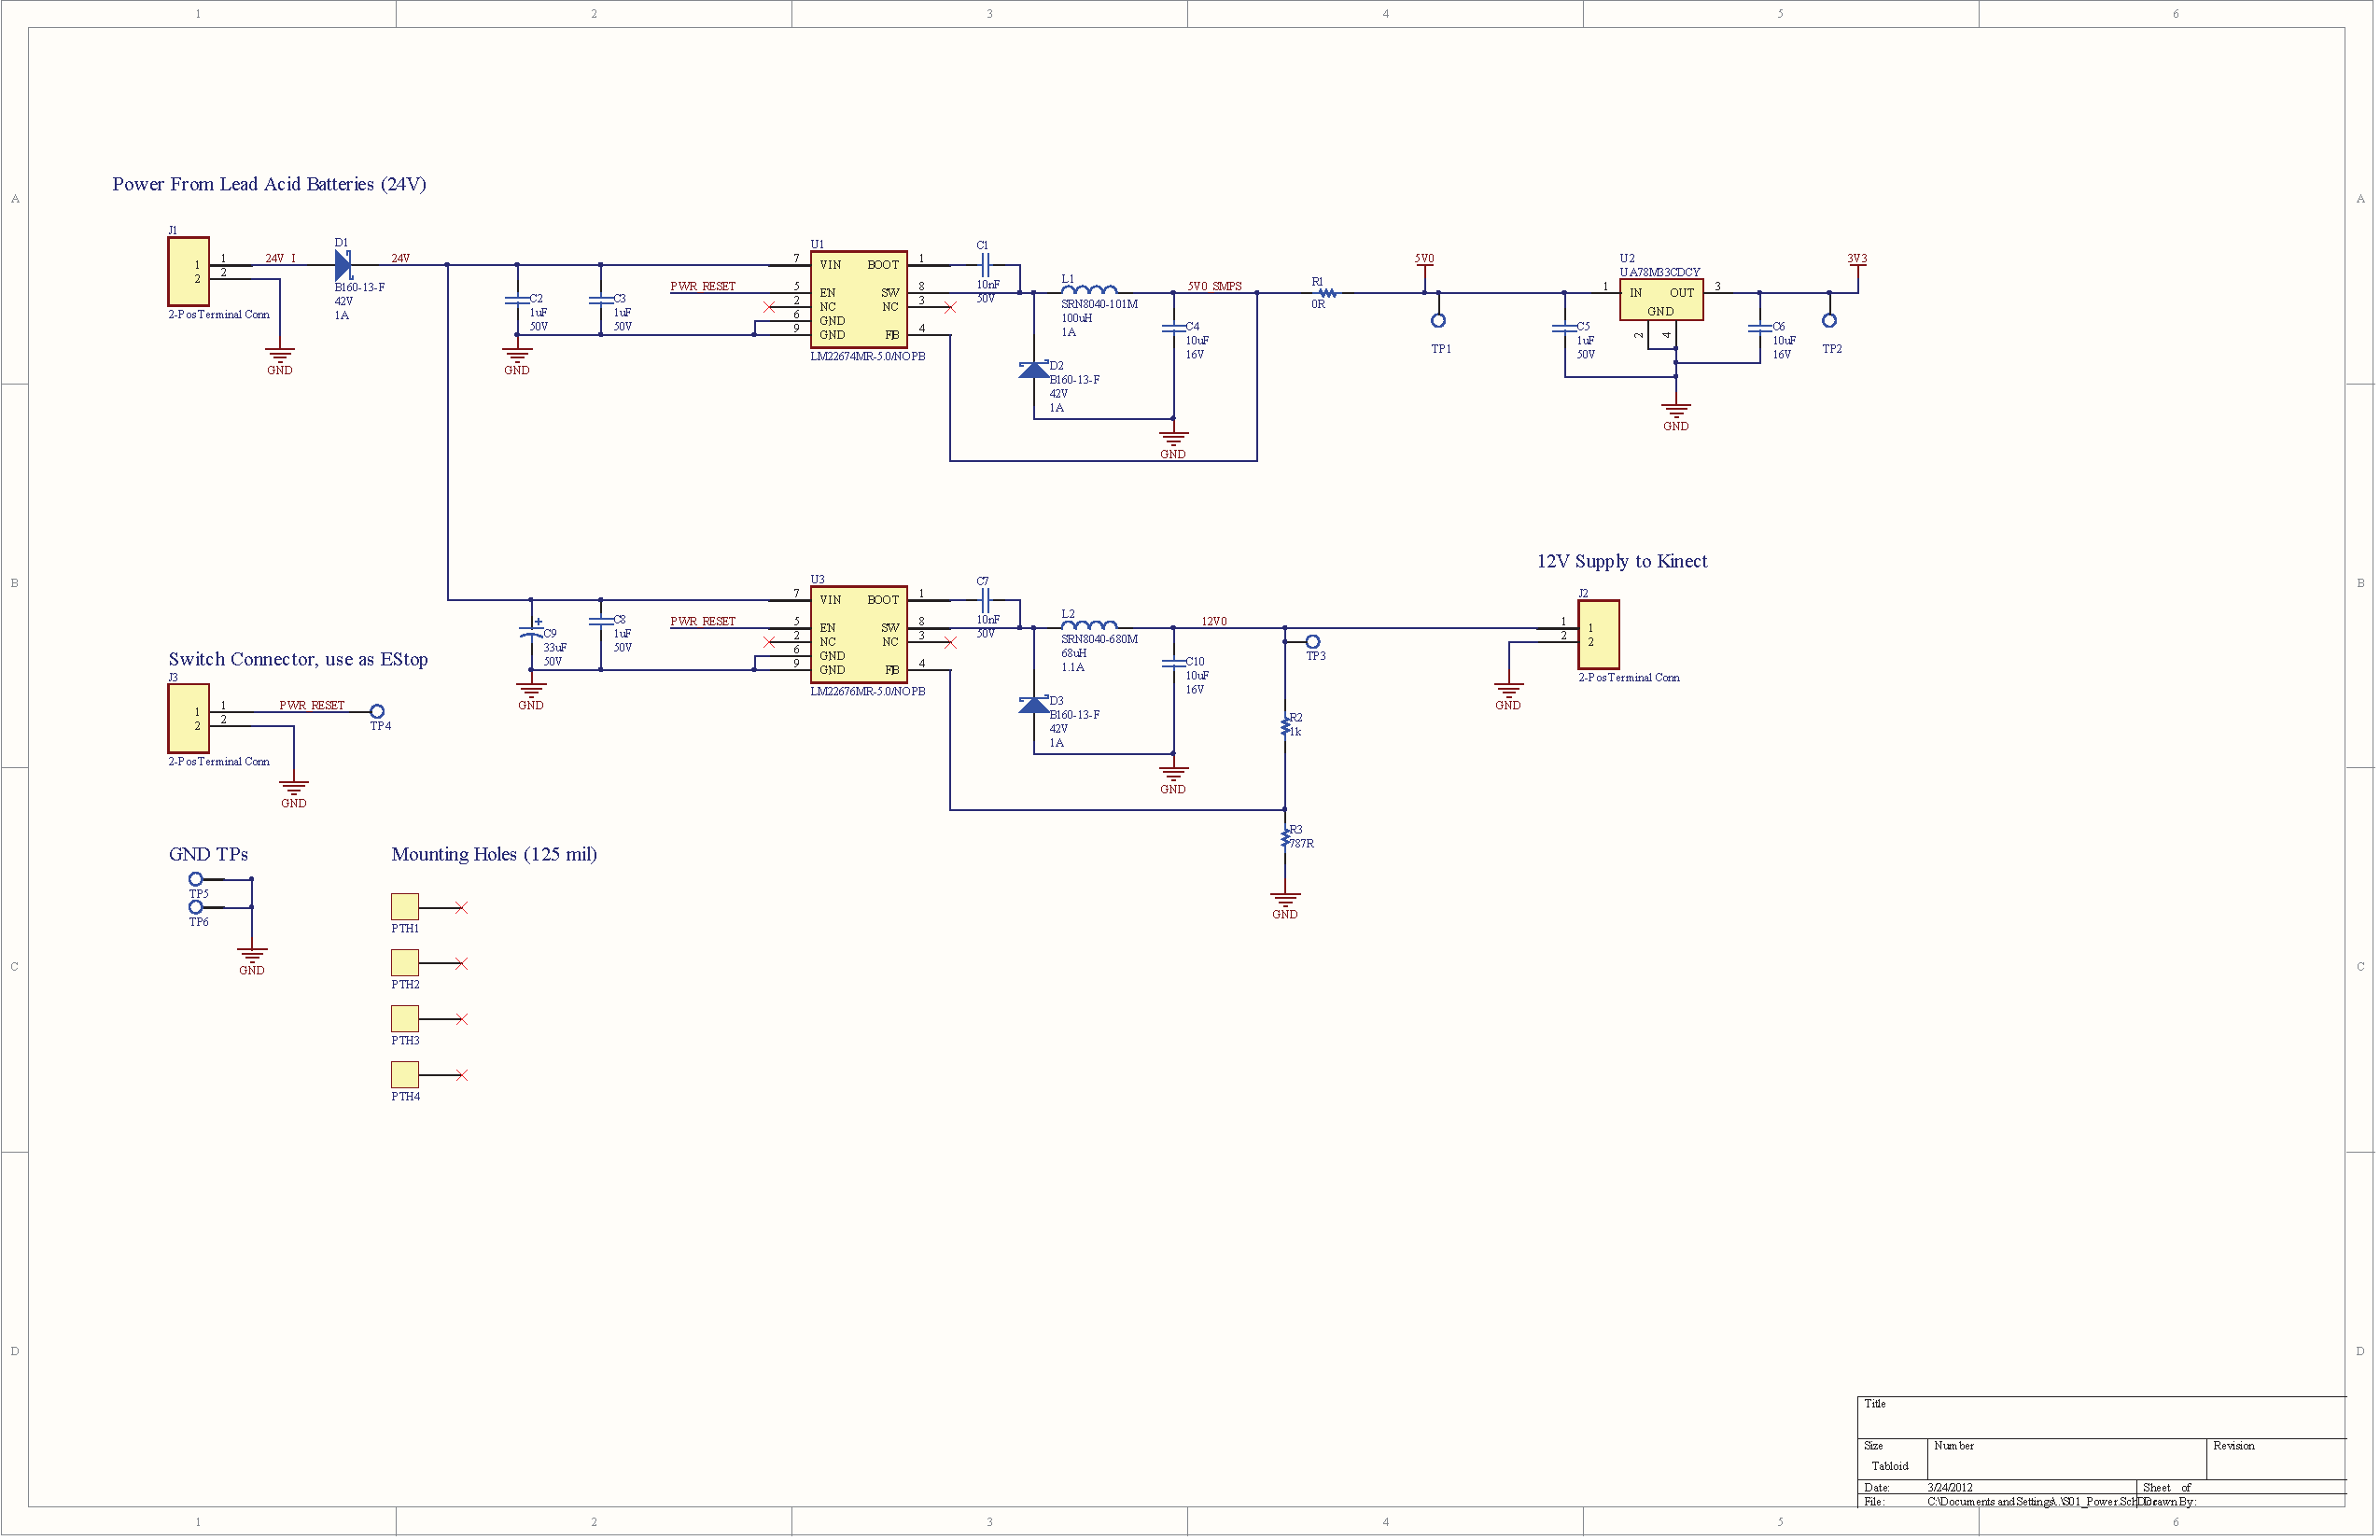
\includegraphics[scale=0.4, angle=270]{FYDP_Schematic_Sheet_1}
\end{figure}
\begin{figure}[hbt]
 \centering
 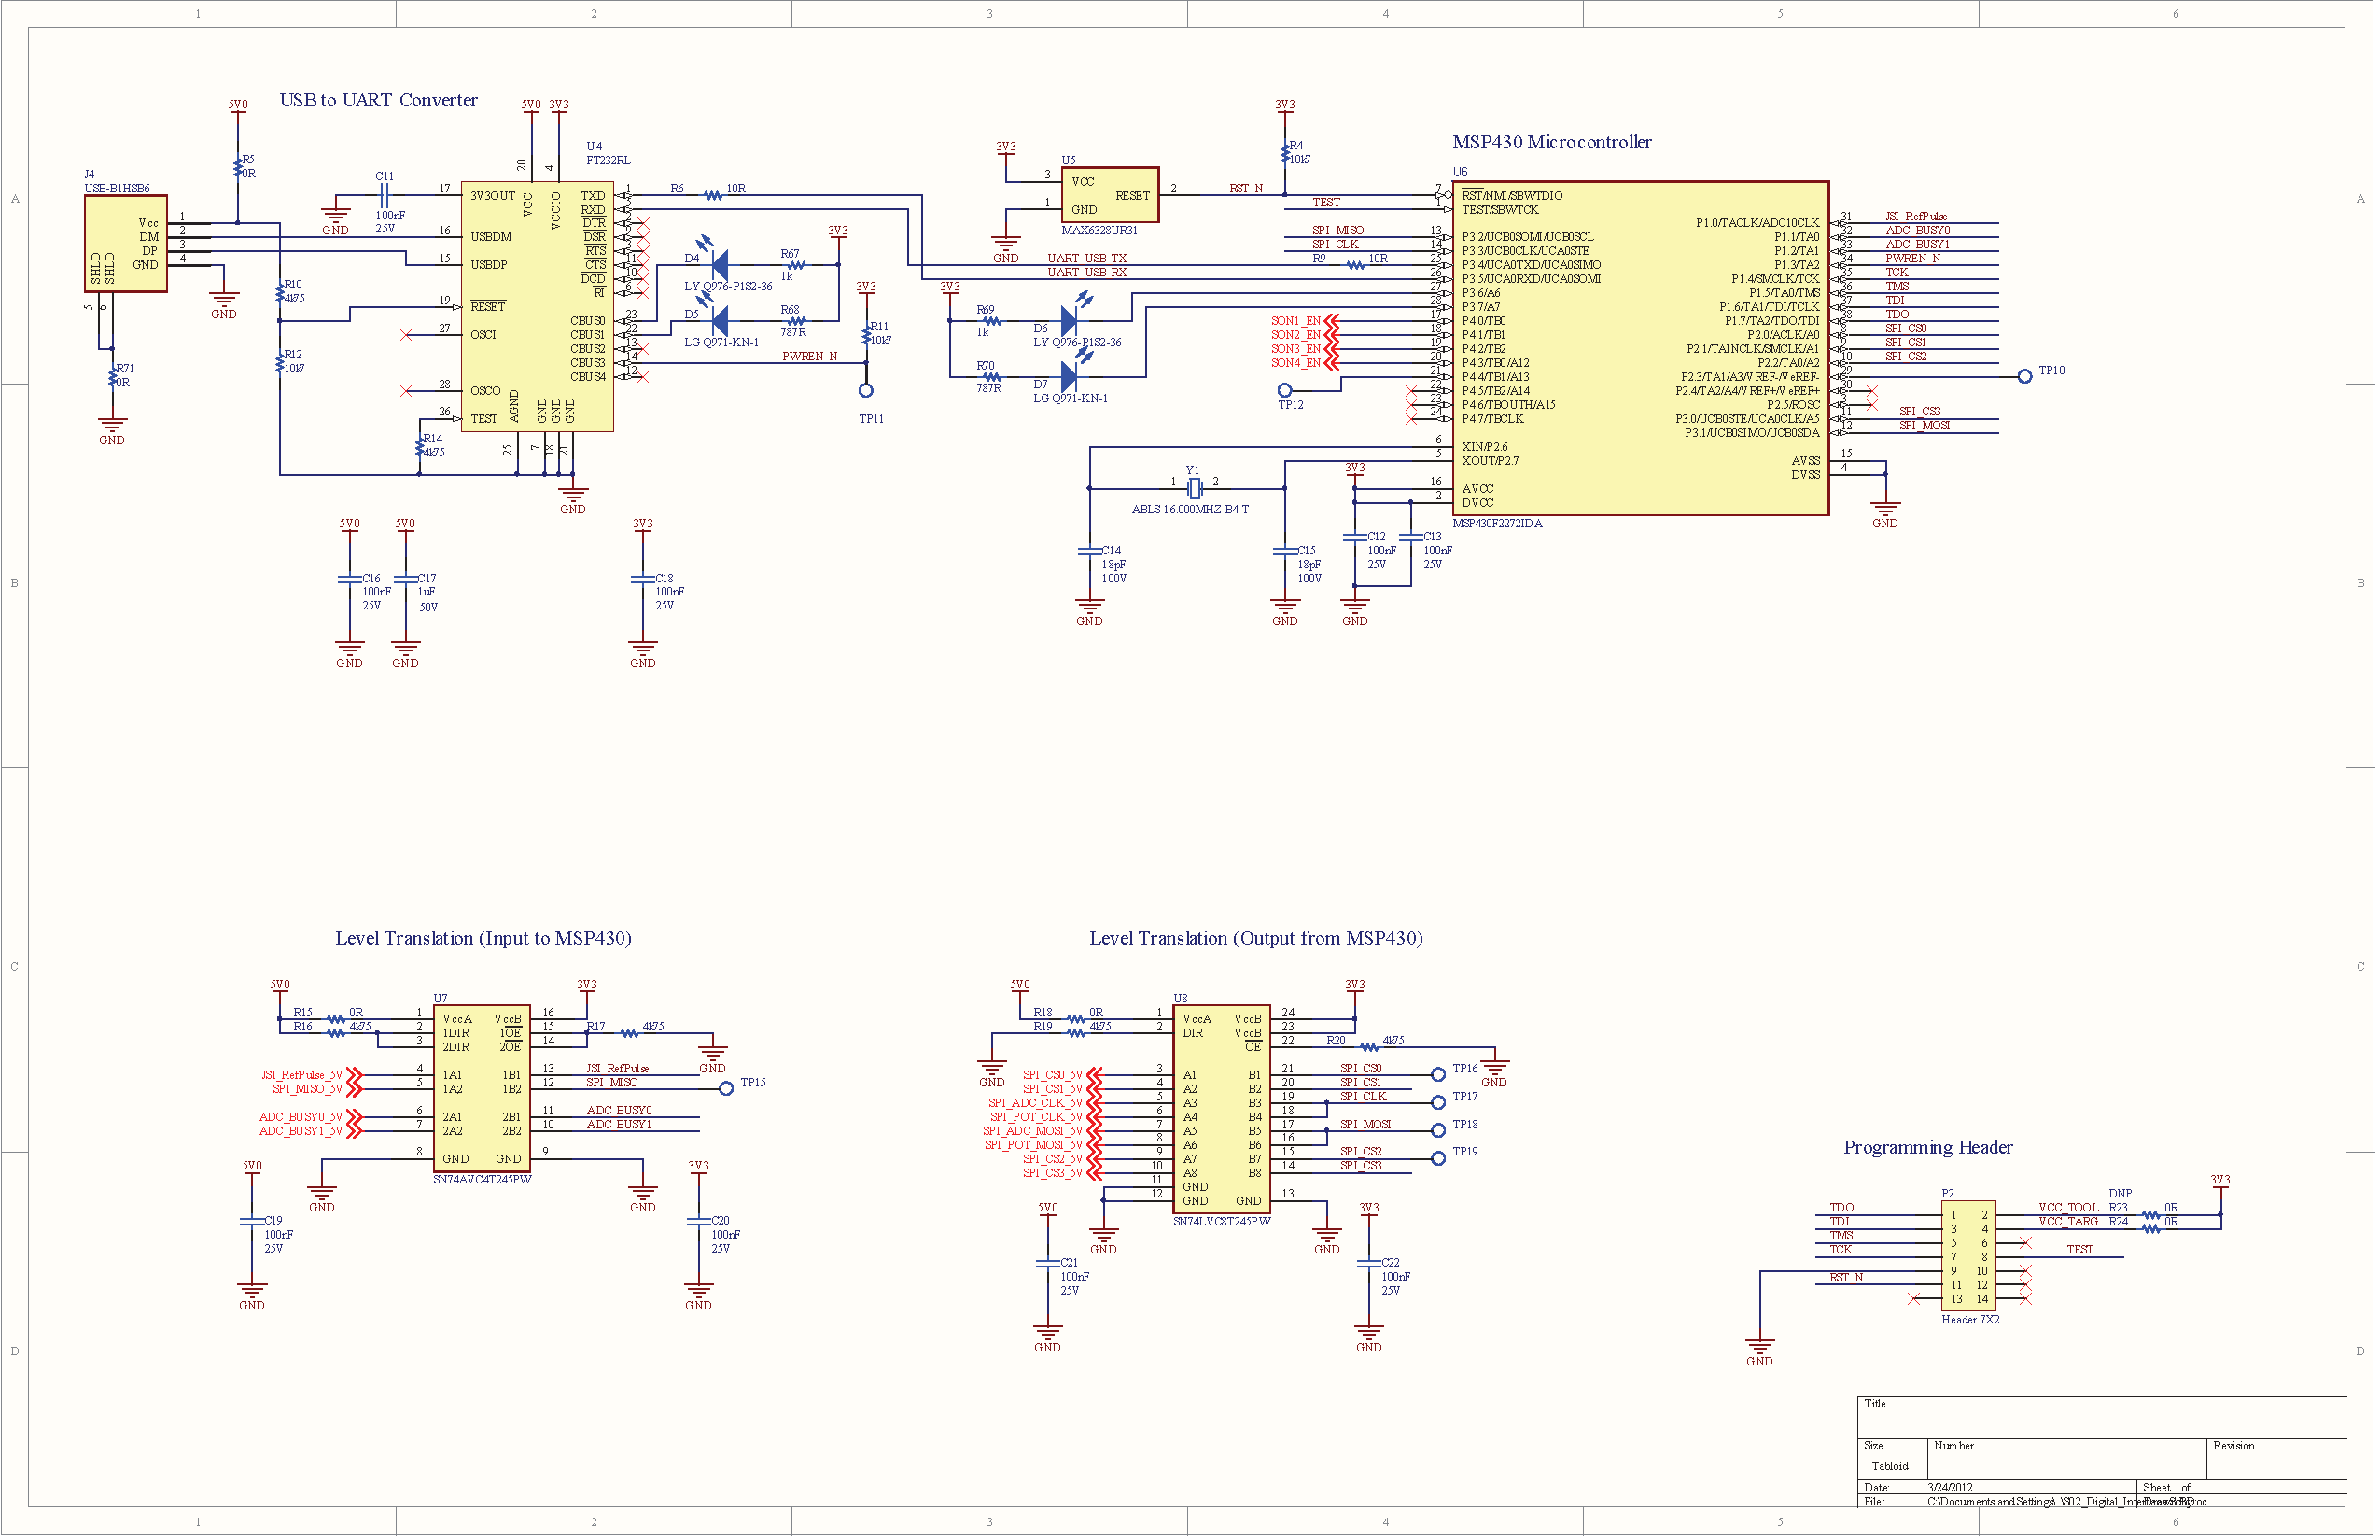
\includegraphics[scale=0.4, angle=270]{FYDP_Schematic_Sheet_2}
\end{figure}
\begin{figure}[hbt]
 \centering
 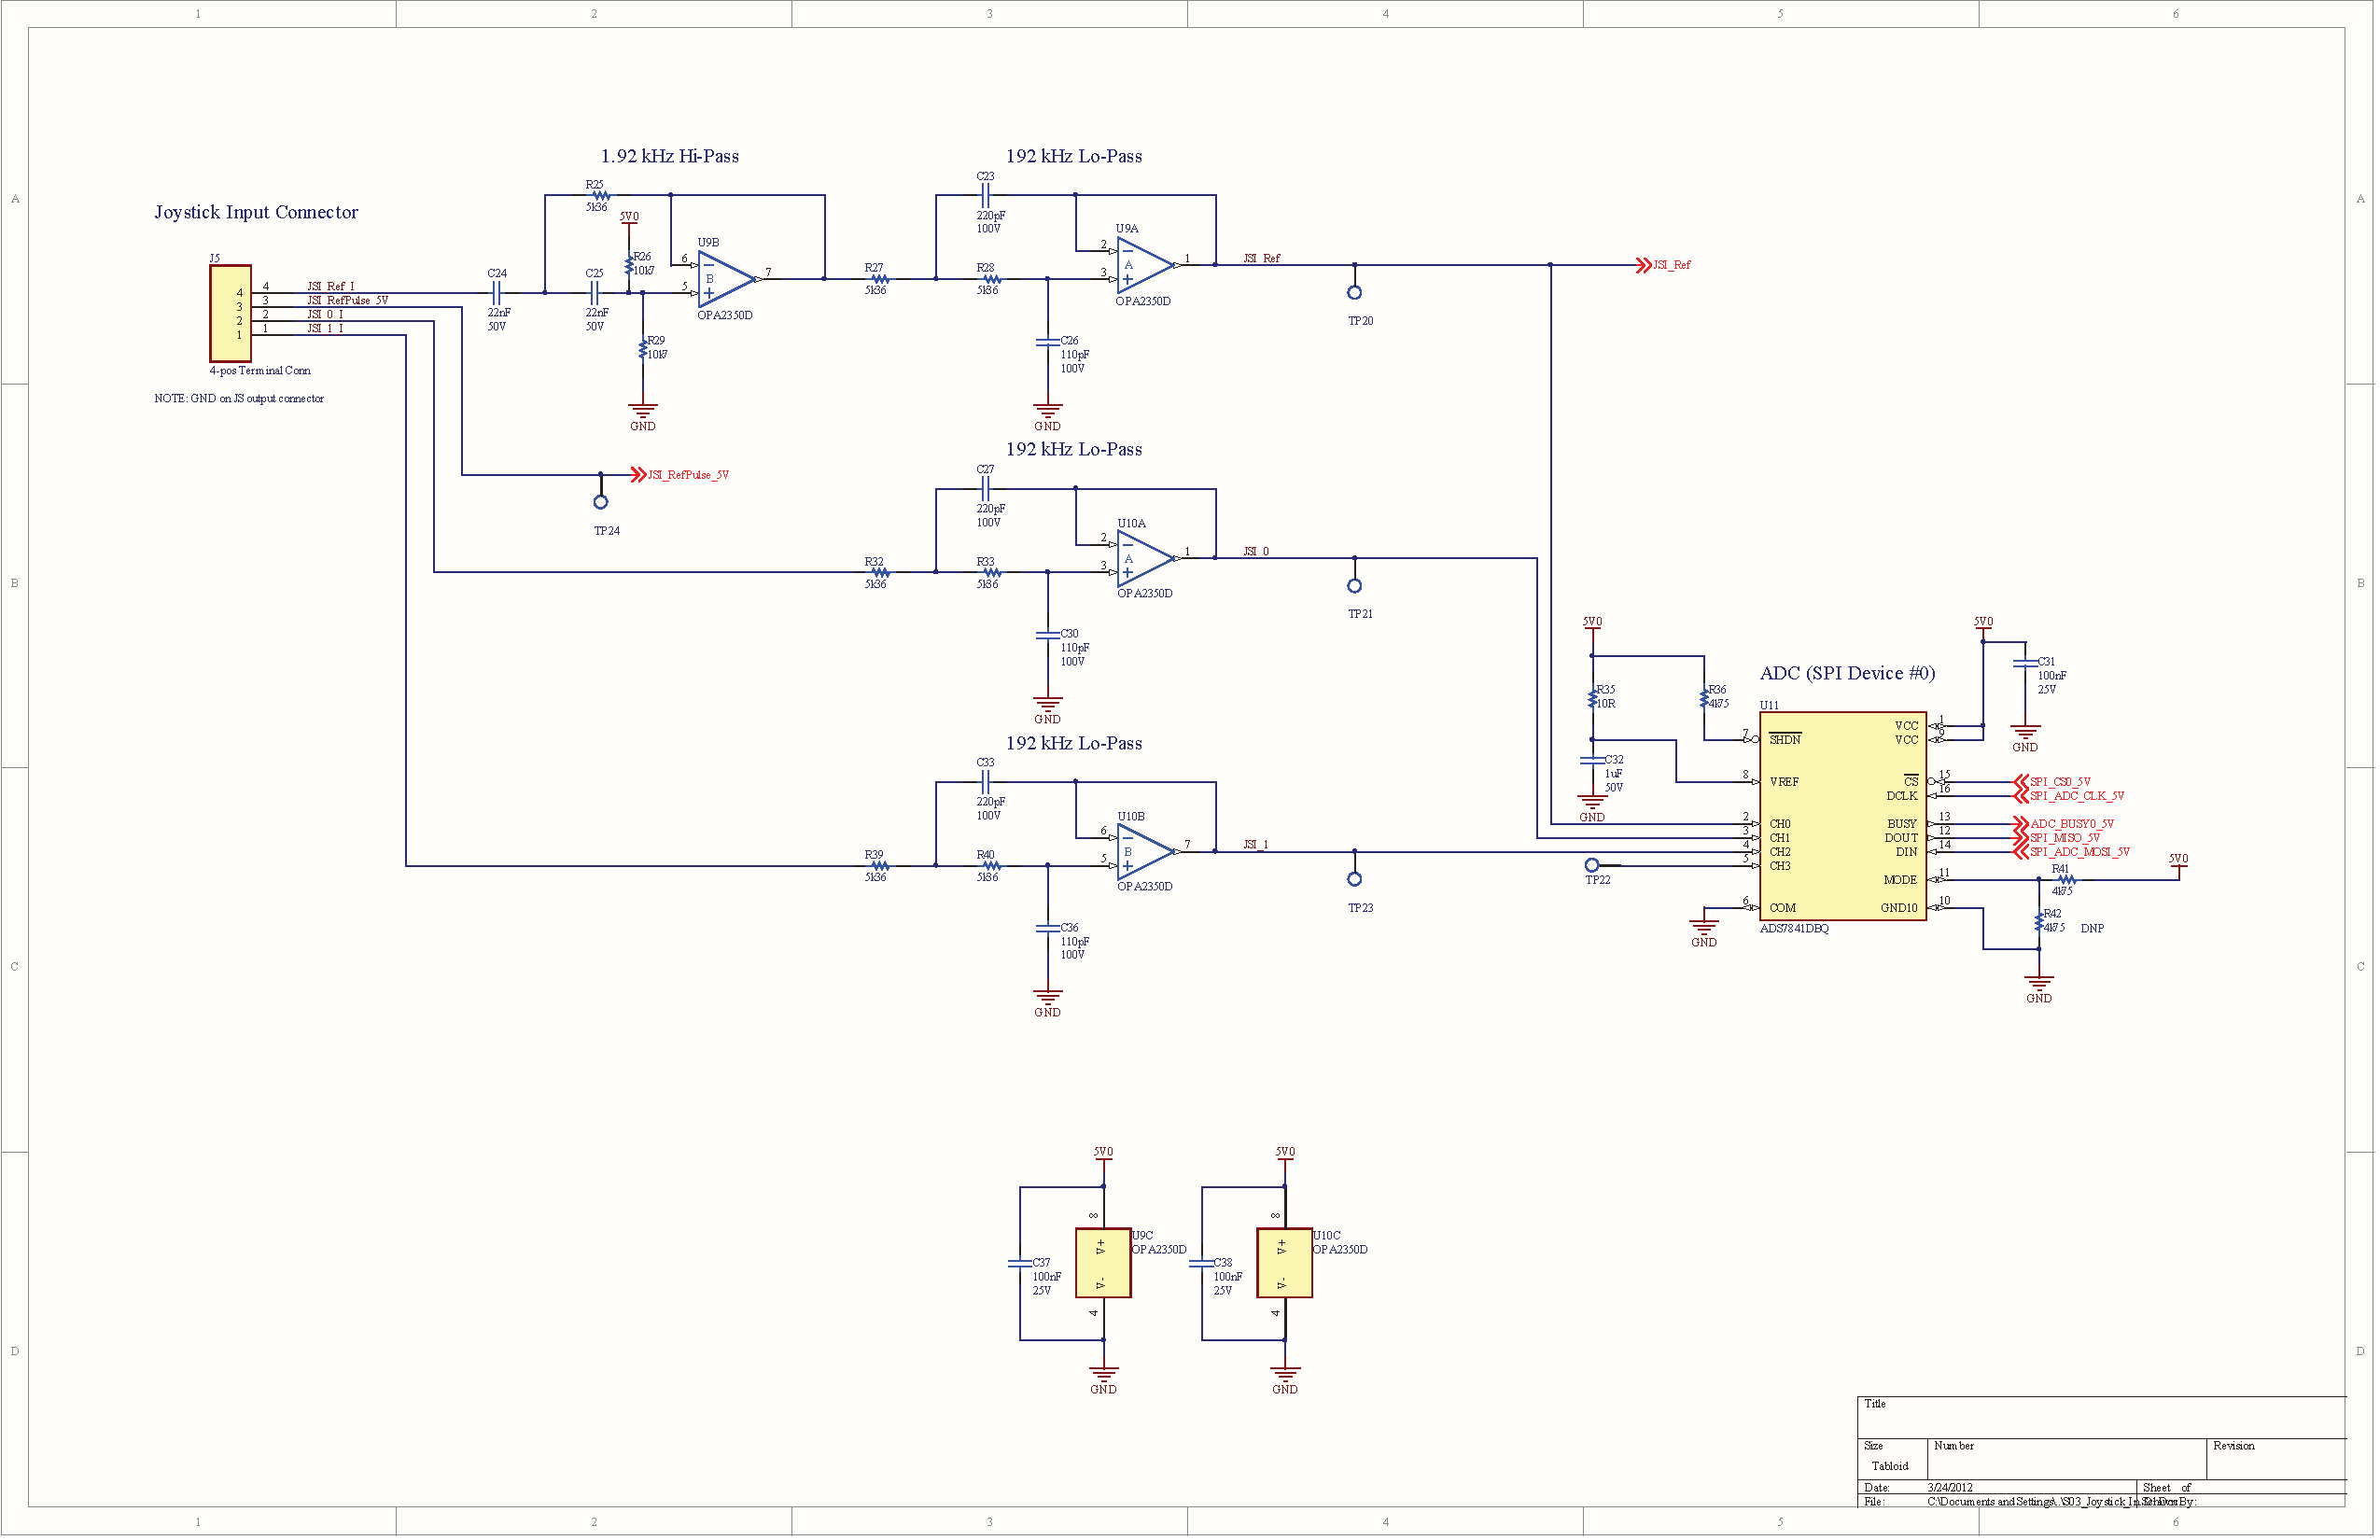
\includegraphics[scale=0.4, angle=270]{FYDP_Schematic_Sheet_3}
\end{figure}
\begin{figure}[hbt]
 \centering
 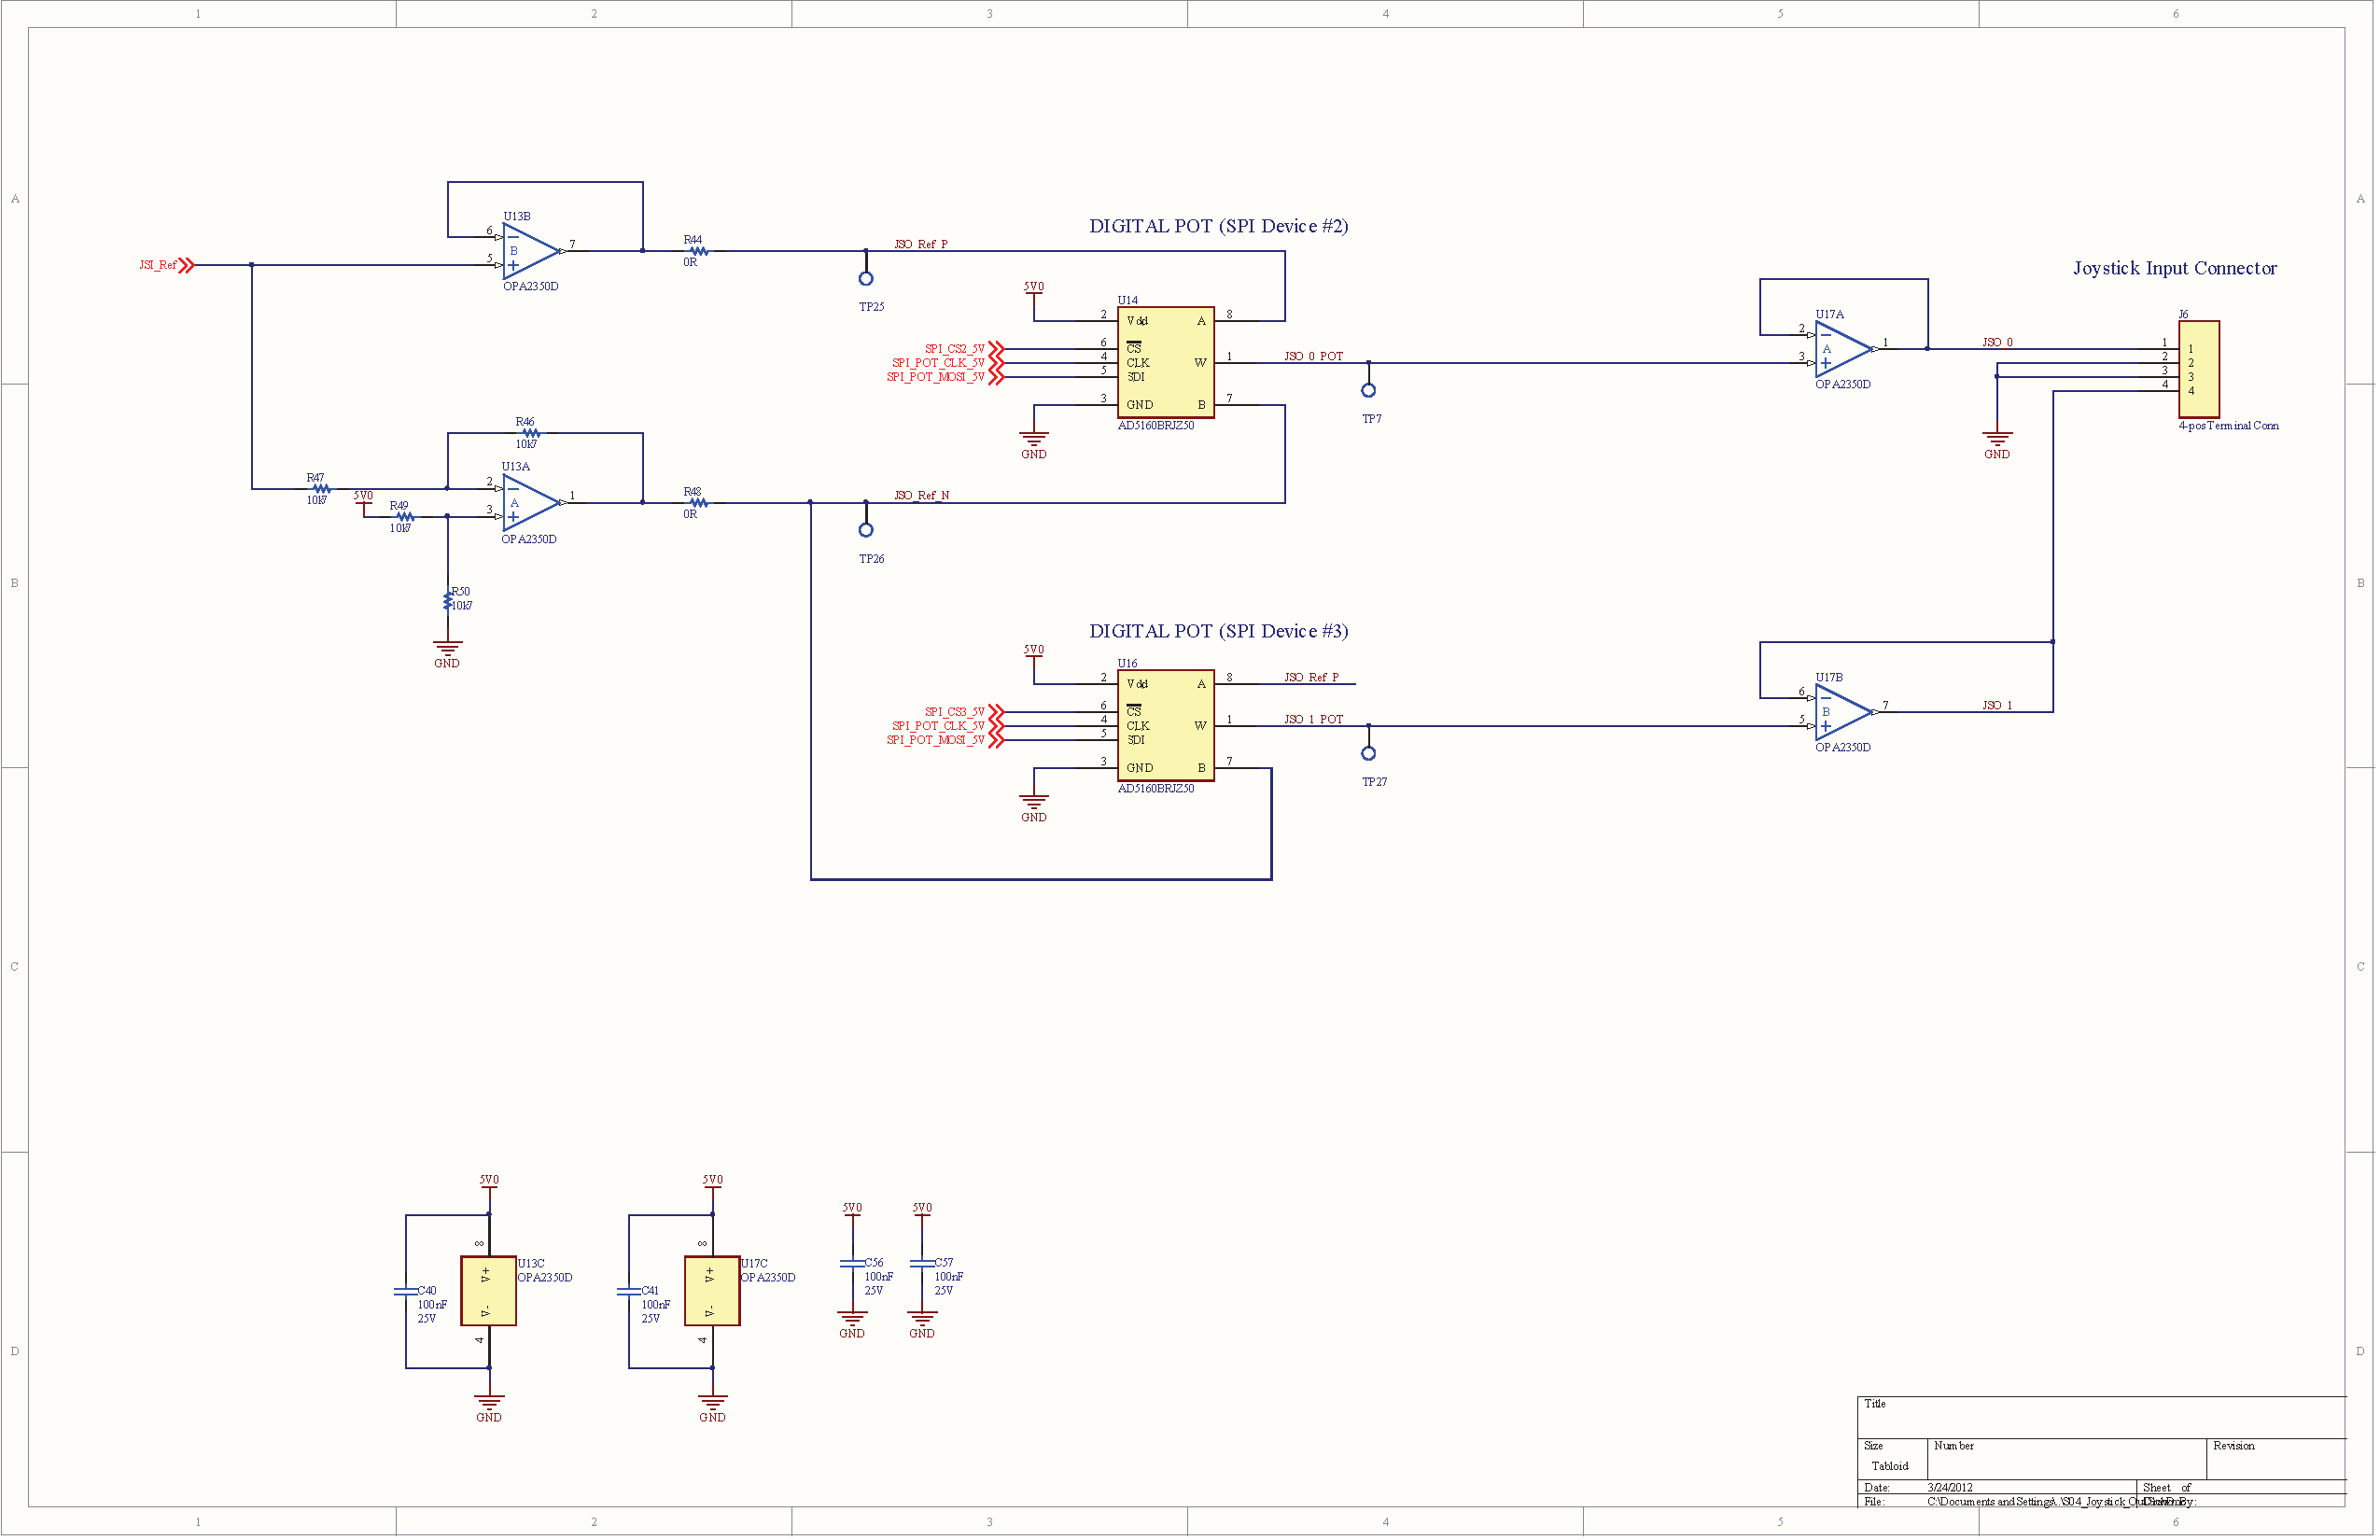
\includegraphics[scale=0.4, angle=270]{FYDP_Schematic_Sheet_4}
\end{figure}
\begin{figure}[hbt]
 \centering
 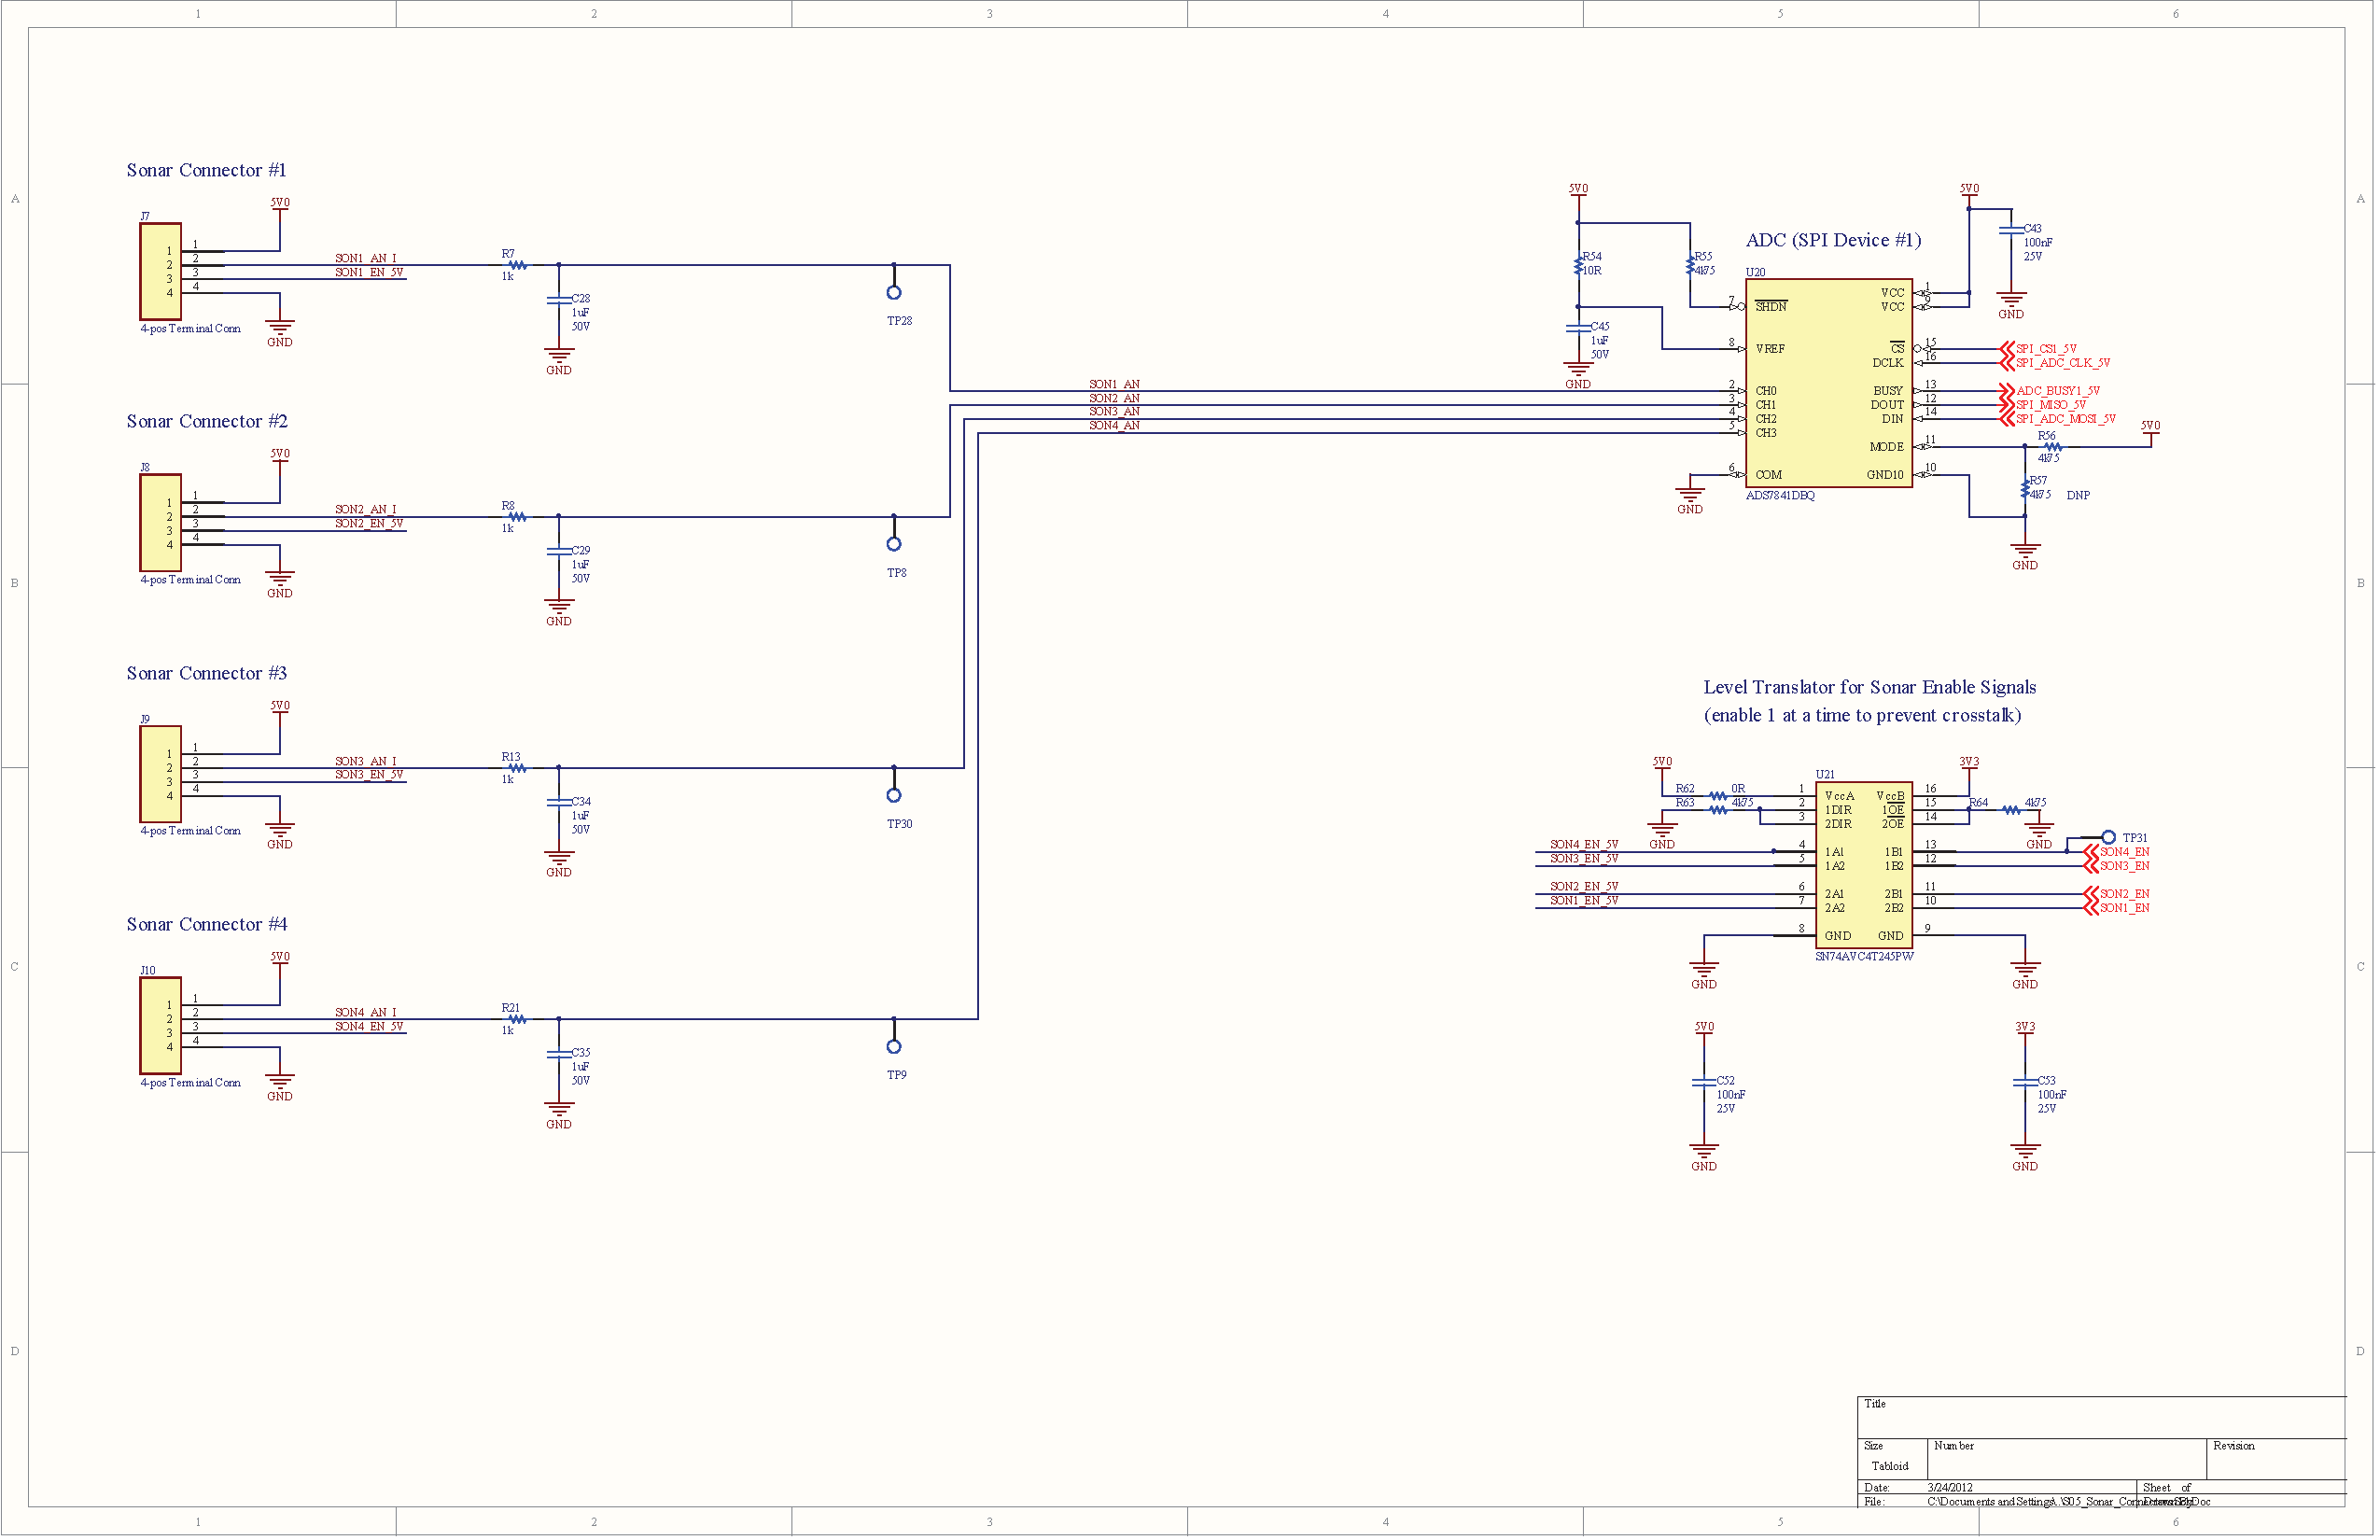
\includegraphics[scale=0.4, angle=270]{FYDP_Schematic_Sheet_5}
\end{figure}

\chapter*{Appendix C - Electrical BOM}
\addcontentsline{toc}{chapter}{Appendix C - Electrical BOM}
\begin{figure}[hbt]
 \centering
 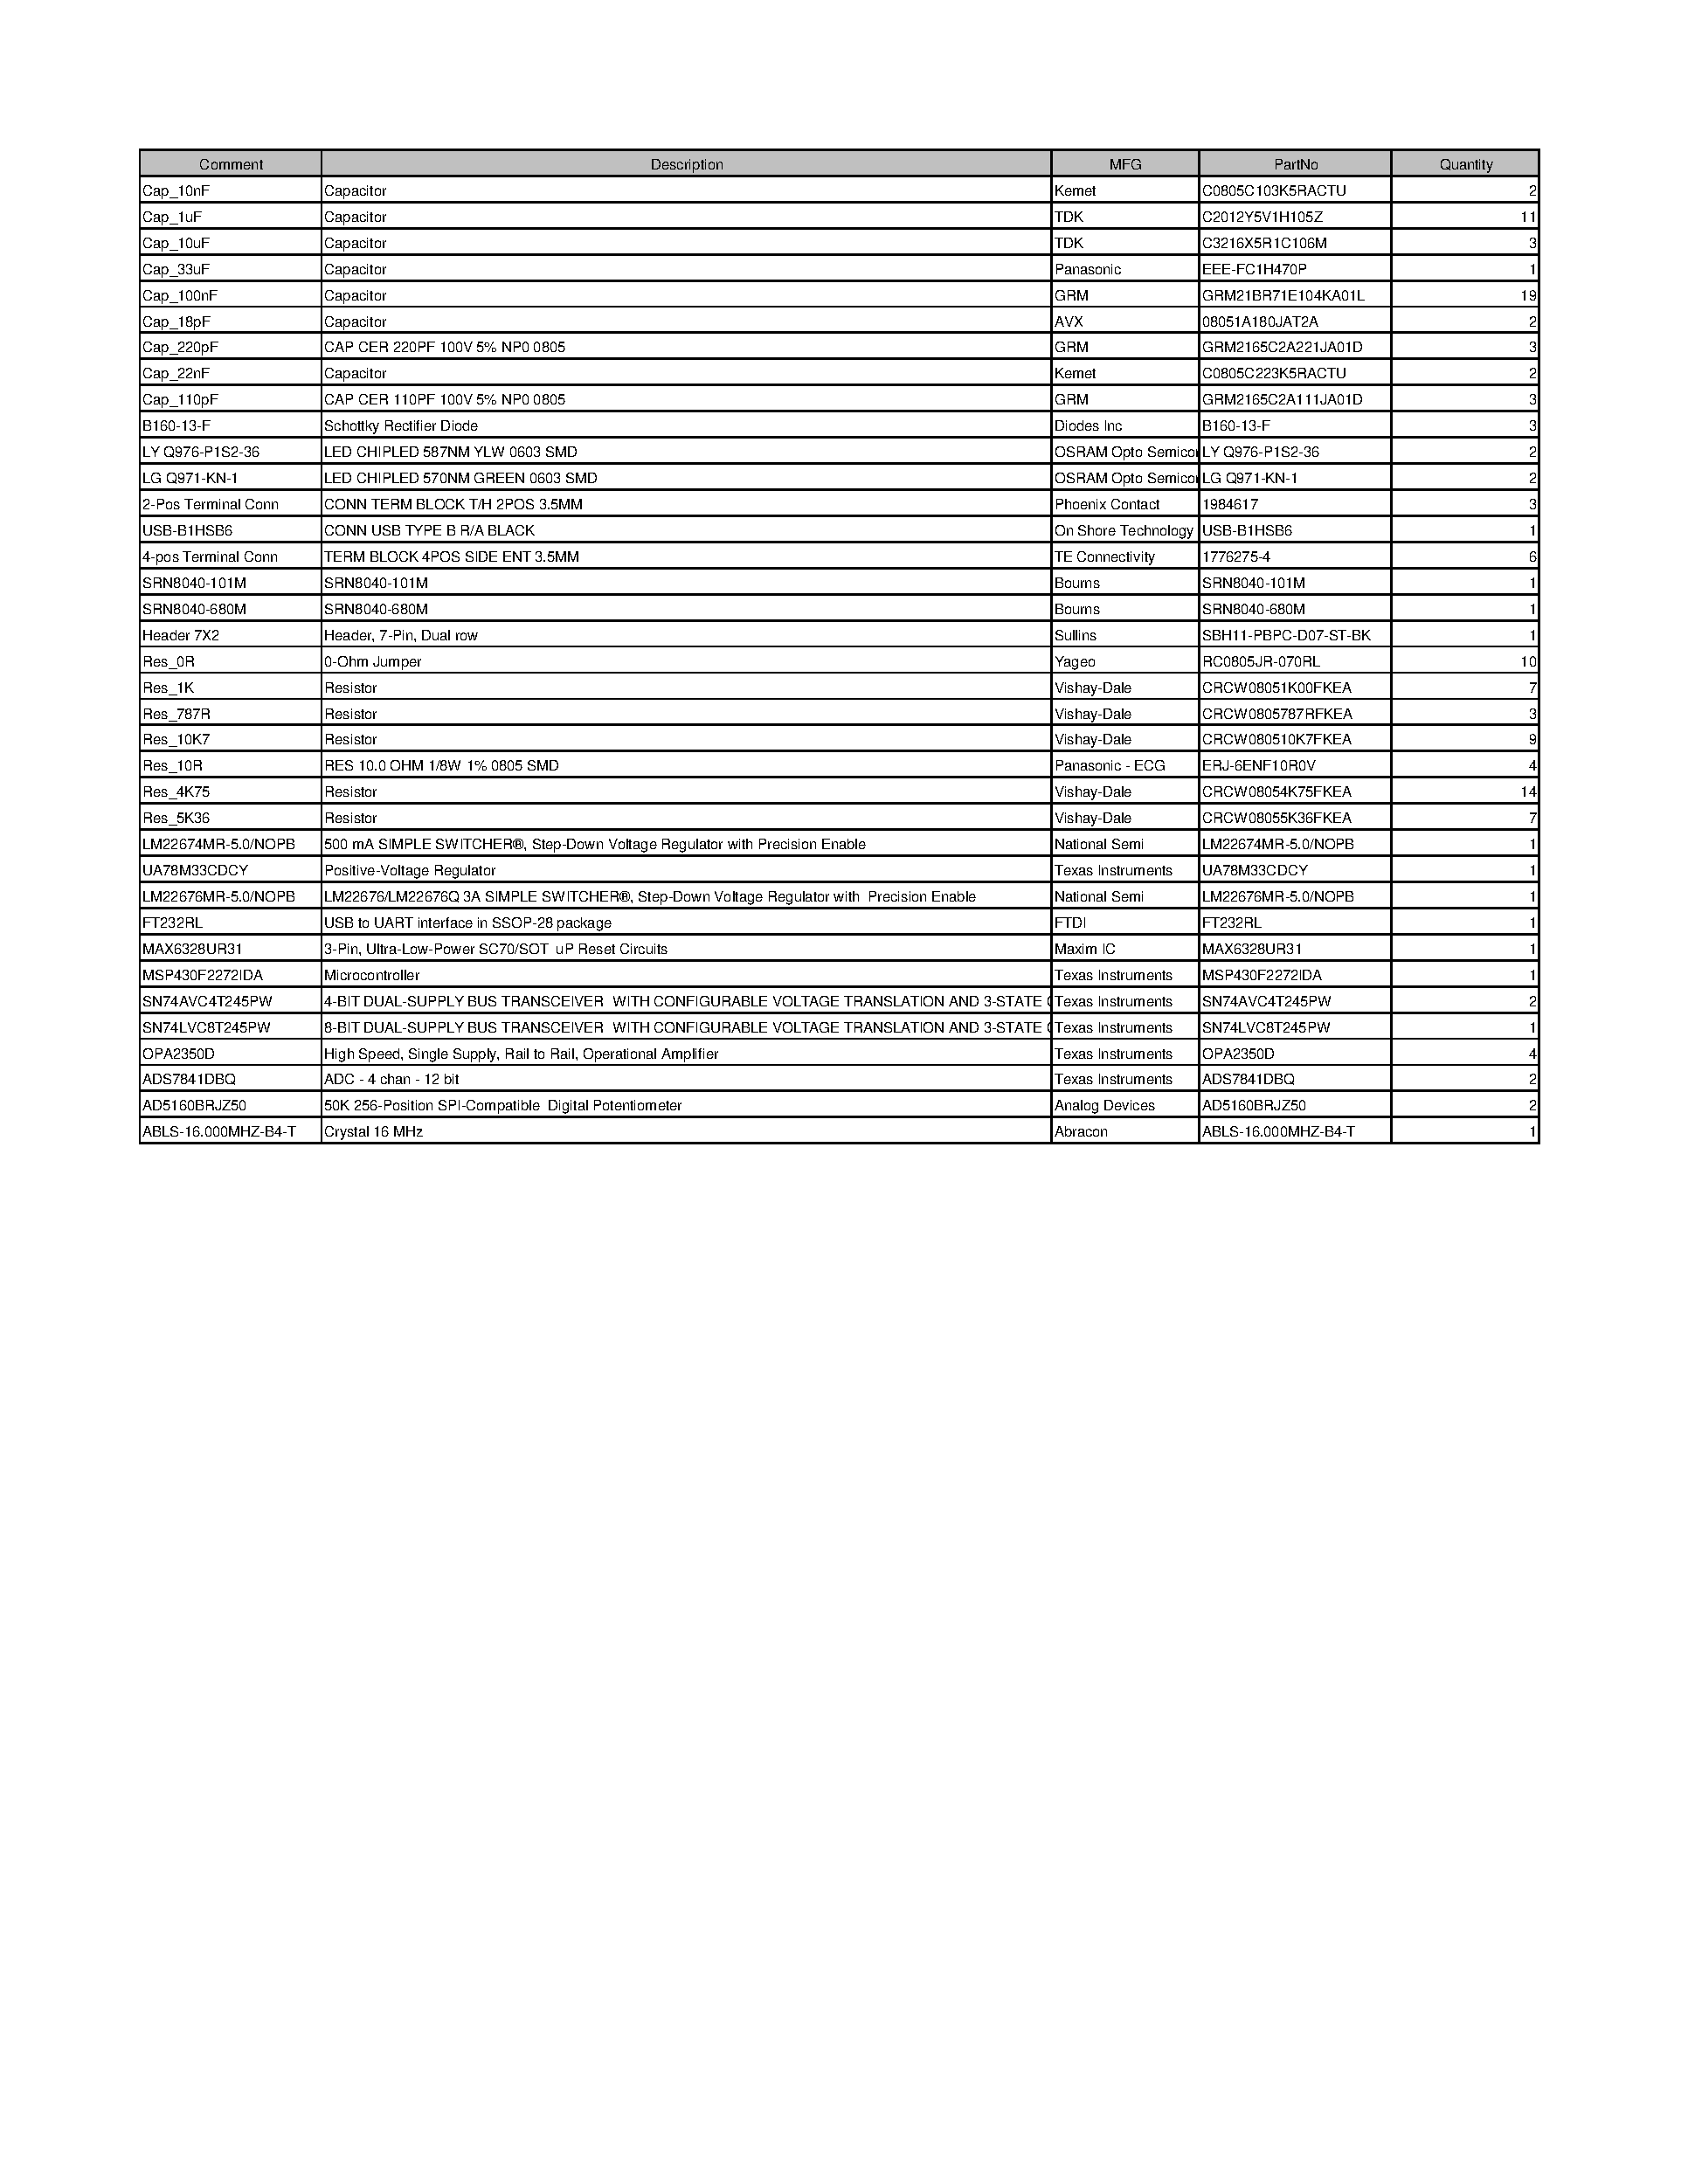
\includegraphics[scale=0.5]{FYDP_BOM}
\end{figure}

\begin{thebibliography}{9}
 \addcontentsline{toc}{chapter}{Bibliography}
 \bibitem{patent:computer_controlled}
  L. Fehr, S. Skaar, G. Del Castillo. \\
  \emph{Computer Controlled Power Wheelchair Navigation System.} \\
  U.S. Patent 2008/7383107B2, Jun. 3, 2008.
 \bibitem{patent:power_wheelchair}
  G. Griggs, T. Dutta, G. Fernie. \emph{Powered Wheelchair},\\
  U.S. Patent 2010/0082182A1, Apr. 1, 2010.
 \bibitem{patent:wheelchair_method}
  T. Smithers, U. Urriticoechea, U. Campos. \\
  \emph{Wheelchair and Method for Correcting the Guidance of a Wheelchair.} \\
  U.S. Patent 2011/0130940A1, Jun. 2, 2011.
 \bibitem{NASA}
  NASA. \emph{NASA-STD-3000. Anthropometry and Biomechanics.}\\
  http://msis.jsc.nasa.gov/sections/section03.htm, Jul. 1995.
\bibitem{primesense}
  \emph{Our Full 3D Sensing Solution}, \\
  \mbox{http://www.primesense.com/en/technology/115-the-primesense-3d-sensing-solution} \\
  2011.
 \bibitem{OpenNI}
  http://www.openni.org/
 \bibitem{ROS}
  http://www.ros.org/
 \bibitem{point_clouds}
  http://pointclouds.org/
 \bibitem{wheelchair_data}
  Invacare. \emph{Nutron R51LXP. Invacare Product Catalogue.} \\
  http://www.invacare.ca/cgi-bin/imhqprd/inv\_catalog/prod\_cat\_detail.jsp?s=0\&prodID=R51LXP\\
 Jan. 2011.
\bibitem{kinect_prec}
  L. Yiping. \\
  \emph{openni\_kinect/kinect\_accuracy}, http://www.ros.org/wiki/openni\_kinect/kinect\_accuracy\\
  Jun. 27, 2011.
 \bibitem{lv-ez4}
  MaxBotix Inc, \emph{LV-EZ4 Datasheet},  2011
 \bibitem{lv-ez0}
  MaxBotix Inc, \emph{LV-EZ0 Datasheet},  2011
 \bibitem{kinect_power}
  M. Wise.  \emph{Adding a Kinect to an iRobot Create} \\
  http://www.ros.org/wiki/kinect/Tutorials/Adding\%20a\%20Kinect\%20to\%20an\%20iRobot\%20Create\\
  May 2, 2011.
 \bibitem{MSP430_USB}
  A. Dannenberg. (2006, October). \emph{MSP430 Connectivity Using TUSB3410},\\
  http://www.ti.com/lit/an/slaa276a/slaa276a.pdf
 \bibitem{kinect_vslam}
  Nicola Fioraio, Kurt Konolige, \emph{Realtime Visual and Point Cloud SLAM}, Willow Garage, 2011
\end{thebibliography}

\end{document}